%--- Load the kaobook class
\documentclass[
	twoside=false, % Use different layouts for even and odd pages (in particular, if twoside=true, the margin column will be always on the outside)
	%open=any, % If twoside=true, uncomment this to force new chapters to start on any page, not only on right (odd) pages
	% secnumdepth=1, % How deep to number headings. Defaults to 1 (sections)
]{kaobook}


% Choose the language
\usepackage[english]{babel} % Load characters and hyphenation
\usepackage[english=british]{csquotes}	% English quotes
\usepackage{mycommands}
\usepackage{mathtools}
\usepackage{preamble}
\usepackage{tikz}
\usepackage[super]{nth}


% Load packages for testing
\usepackage{blindtext}
%\usepackage{showframe} % Uncomment to show boxes around the text area, margin, header and footer
%\usepackage{showlabels} % Uncomment to output the content of \label commands to the document where they are used

% Load the bibliography package
\usepackage{kaobiblio}
\addbibresource{symlinks/zotero-library-automatic-export.bib} % Bibliography file

\usepackage{xcolor}
\definecolor{def}{HTML}{F8EBFF}
\definecolor{thm}{HTML}{FFF7D9}
\definecolor{cor}{HTML}{EEFFE0}
% Load mathematical packages for theorems and related environments
\usepackage[
  framed=true,
  theorembackground=thm,
  lemmabackground=thm,
  propositionbackground=thm,
  definitionbackground=def,
  corollarybackground=cor
  ]{kaotheorems}

% Load the package for hyperreferences
\usepackage{kaorefs}

\graphicspath{{images/}{./}{symlinks/illustrations}} % Paths where images are looked for

% \makeindex[columns=3, title=Alphabetical Index, intoc] % Make LaTeX produce the files required to compile the index

\usepackage{subfiles} % Best loaded last in the preamble

\setcounter{tocdepth}{1}

\begin{document}

\pagelayout{wide}
\begin{titlepage}
  \pagelayout{wide} % No margins
  \begin{center}
    {\LARGE \textbf{Model Correlation in Random Forests}}
    \\[2em]
    {\Large {Master Thesis}}
    \\[5.5em]
    {\Large presented by}
    \\[1.5em]
    {\LARGE \textbf{Benjamin Moser}}
    \\[1.5em]
    {\Large at the}
    \\[1.2em]
    % TODO signet
    % TODO faculty
    {\Large \textbf{University of Konstanz}}
    \\[1.0em]
    {\Large \textbf{Department of Computer and Information Science}}
    \\[4em]
    \begin{align*}
      % TODO check titles
      % TODO fix issues with nth
      % \text{\large {\nth{1} Supervisor}:~} &  \text{ \large Prof.\ Dr.\ Sven Kosub } \\
      % \text{\large {\nth{2} Supervisor}:~} &  \text{ \large Prof.\ Dr.\ Tobias Sutter } \\
    \end{align*}
    \vfill
    {\Large {Konstanz, 2023}}
  \end{center}
\end{titlepage}

% \begin{center}
% {\LARGE \textbf{Model Correlation in Random Forests}}
% \\[1cm]
% {\Large \textbf{Master Thesis}}
% \\[1cm]
% {\Large presented by}
% \\[0.5cm]
% {\LARGE \textbf{Benjamin Moser}}
% \\[0.5cm]
% {\Large at}
% \\[0.5cm]
% \includegraphics[width=0.4\textwidth]{pics/unisignet-klein.jpg}
% \\[1cm]
% {\Large \textbf{Faculty of Sciences}}
% \\[1cm]
% {\Large \textbf{Department of Computer and Information Science}}
% \\[2cm]
% \begin{minipage}[c]{0.8\textwidth}
% \begin{description}[style=multiline]
%  % TODO 1st, 2nd
%  % TODO check titles
%  \item {\Large \textbf{1. Advisor:} Prof. Dr. Sven Kosub}
%  \item {\Large \textbf{2. Advisor:} Prof. Dr. Tobias Sutter }
% \end{description}
% \end{minipage}
% \vfill
% {\LARGE \textbf{Konstanz, 2023}}
% \end{center}
% \pagelayout{margin}
% \end{titlepage}

%----------------------------------------------------------------------------------------
%	BOOK INFORMATION
%----------------------------------------------------------------------------------------

% \titlehead{Document Template}
\title[Model Correlation in Random Forests]{Model Correlation in Random Forests}
\author[BM]{Benjamin Moser}
\date{\today}
% \publishers{An Awesome Publisher}

%----------------------------------------------------------------------------------------

\frontmatter % Denotes the start of the pre-document content, uses roman numerals


%----------------------------------------------------------------------------------------
%	OUTPUT TITLE PAGE AND PREVIOUS
%----------------------------------------------------------------------------------------

% Note that \maketitle outputs the pages before here
% \maketitle



%----------------------------------------------------------------------------------------
%	PREFACE
%----------------------------------------------------------------------------------------

\chapter*{Abstract}

...

%----------------------------------------------------------------------------------------
%	TABLE OF CONTENTS & LIST OF FIGURES/TABLES
%----------------------------------------------------------------------------------------

\begingroup % Local scope for the following commands

% Define the style for the TOC, LOF, and LOT
%\setstretch{1} % Uncomment to modify line spacing in the ToC
%\hypersetup{linkcolor=blue} % Uncomment to set the colour of links in the ToC
\setlength{\textheight}{230\vscale} % Manually adjust the height of the ToC pages

% Turn on compatibility mode for the etoc package
\etocstandarddisplaystyle % "toc display" as if etoc was not loaded
\etocstandardlines % "toc lines as if etoc was not loaded

\tableofcontents % Output the table of contents

% \listoffigures % Output the list of figures

% Comment both of the following lines to have the LOF and the LOT on different pages
\let\cleardoublepage\bigskip
\let\clearpage\bigskip

% \listoftables % Output the list of tables

\endgroup

%----------------------------------------------------------------------------------------
%	MAIN BODY
%----------------------------------------------------------------------------------------

\mainmatter % Denotes the start of the main document content, resets page numbering and uses arabic numbers

%wider contents, more narrow margins
\renewcommand{\marginlayout}{%
 \newgeometry{
	top=27.4mm,
	bottom=27.4mm,
	inner=24.8mm,
	textwidth=127mm, % increased
	marginparsep=5.2mm,
	marginparwidth=39.4mm 
 }%
}
\pagelayout{margin}

\setchapterstyle{plain} % Choose the default chapter heading style

\chapter{Introduction}

% TODO argue why we are considering the combination of diversity theory and random forests -- in that it is particularly relevant there
% cf also homog ensembles, avg bias equals ens bias? could imply the variance reduction through ens improvement

\section{Overview}

% TODO use the below text as basis?

% Es geht um Ensemble Learning am Beispiel von Random Forests. Das "klassische" Verständnis ist, dass die Kombination von einzelnen Lernern (zB Entscheidungsbäumen) eine niedrigere Varianz (im Sinne von Bias-Variance-Tradeoff) zeigt als der durchschnittliche einzelne Lerner. Weiter hängt das Ausmaß dieser Verbesserung davon ab, wie ähnlich die Vorhersagen der einzelnen Lerner sind. Solche Aussagen wurden allerdings klassischerweise hauptsächlich spezifisch für den Squared-Error-Loss gezeigt. 

% In meiner Arbeit geht es nun zuerst einmal darum, zu verstehen welche Faktoren genau den Fehler eines Ensembles wie beeinflussen. Dazu behandle ich zunächst einmal eine gewisse Theorie (https://arxiv.org/abs/2301.03962), die sich erst in den letzten 1-2 Jahren herausgebildet hat. Das hauptsächliche Ergebnis ist (a) eine allgemeine Bias-Variance-Zerlegung für jeden Loss, (b) eine allgemeine "Ambuigity"-Zerlegung, die die Unterschiede zwischen den einzelnen Lernern berücksichtigt und (c) als Kombination von (a+b) eine eine (exakte) Zerlegung des Ensemble-Fehlers in durschnittlichen Bias der Lerner, durchschnittliche Varianz und ein Maß von *Diversität* zwischen den einzelnen Lernern. 

% Für Bregman Divergences, zu denen u.a. Squared Error und KL-Divergence zählen, vereinfacht sich diese allgemeine Form und es zeigt sich, dass diverse Resultaet, die für spezielle Loss-Funktionen gezeigt wurden, Spezialfälle dieser allgemeinen Struktur sind. Der 0/1-Loss allerdings zählt hier nicht dazu. Hier können wir aber trotzdem noch auf die allgemeine Form der Zerlegung zurückgreifen. 

% Für diese Zerlegungen gebe ich einen alternativen Beweis.

% Ausgehend davon betrachte ich dann Wachstumsstrategien für Ensembles. Eine grundliegende Einsicht ist u.a., dass -- genau wie Bias und Varianz -- die Diversität punktweise gemessen wird ("Erwartungswert über X"). An unterschiedlichen Punkten trägt die Diversität unterschiedlich zum übergreifenden Ensemble-Fehler bei. Insbesondere für Klassifikation unter dem 0/1-Loss ergibt sich hier eine klare binäre Unterscheidung in positiven und negativen Beitrag. Es zeigt sich also, dass Diversität nicht immer vorteilhaft ist, sondern nur an bestimmten Punkten. Dadurch motiviert betrachte ich eine gewisse Wachstumsstrategie, die Diversität an "positiven" Punkten steigert und an "negativen" Punkten verringert. Dies lässt sich wahrscheinlich auch auf das Regressionsproblem übertragen.

% Eine bereits bekannte Wachstumsstrategie für Ensembles von neuronalen Netzen ist "Negative Correlation Learning". Darin wird eben auch Diversität zwischen den einzelnen Lernern erzeugt. Es gab in der Vergangenheit einige Versuche, NCL, ursprünglich für den Squared Error Loss definiert, zu verallgemeinern. Ich argumentiere, dass die obengenannte Zerlegung eine natürliche Verallgemeinerung ist.

\section{Contributions}

% Can motivate many of the choices in decision tree learning from the perspective of bregman divergences

% Alternate proof of the classic bias-variance-decomposition via effect-decompositions and Bregman divergences. This shows that it is but an example for a much broader structure and gives much clearer intuition (instead of just doing the magic in the direct proof).

% Insight that exploiting diversity has to happen through doing so at places where we can \textit{afford} to do so -- i.e. "without affecting bias too much".

% TODO more


\section{Statistics}

% TODO maybe remove probability space etc definitions and just assume expected value is known.
We want to reason in a general manner about algorithms which act on data. We use statistical language for this. Consider a data point $X$ that is provided as input to an algorithm. Our intention is to say that $X$ could be essentially \textit{any} data point from some kind of data source. In other words, we can consider $X$ to be \textit{random}, that is, $X$ is a random variable (a symbol) that can take different values. 
Which values exactly it can take depends on the data source -- the \textit{distribution} of the data. If our data source is a fair $6$-sided die, $X$ can take values in $\Omega = \{ 1, \dots, 6 \}$ and the distribution of values is constant where each outcome has probability $\frac{1}{6}$, i.e. $\prob{}{1} = \dots  = \prob{}{6} = \frac{1}{6}$.
\marginnote{
    A
      \(\sigma\)-algebra over \(\Omega\) can be thought of a set of subsets of
      \(\Omega\), containing \(\Sigma\), such that it is closed under complement
      and countable union and intersection.
}
\begin{definition}
  A \textit{probability space} is a triple \((\Omega, \Sigma, \mathbb{P})\)
  where
  \begin{itemize}
  \item \(\Omega\) is an arbitrary set modelling the \textit{sample space}
    i.e.~the set of all possible outcomes.
  \item \(\Sigma\) is a \(\sigma\)-algebra
    over \(\Omega\), modelling the set of \textit{events}.
    \item \(\mathbb{P}\) is a function
    \(\Sigma \to [0,1]\) such that \(\mathbb{P}(\Omega)=1\) and
    \(\mathbb{P}\left( \bigcup_{i=1}^\infty A_{i} \right) = \sum_{i=1}^\infty
    \mathbb{P}(A_{i})\) for a countable collection of (pairwise disjoint) sets
    in \(\Sigma\), and models the \textit{probability measure}.
  \end{itemize}
\end{definition}
In the following, we assume an underlying probability space implicitly.
% def random variable
\begin{definition}
  A \textit{random variable} is a quantity
  that depends on a random event, i.e. a function \(\Omega
  \to M\) (commonly, we have \(M=\mathbb{R}\)).
  % that assigns a value to each outcome.
\end{definition}
Further, we not only want to reason about the behaviour of an algorithm with respect to one point $X$ but many such points. A basic notion is the \textit{expected value} of $X$. Further, since $X$ is considered random, $f(X)$ is also a random variable and we can talk about the expected value of functions of random variables.
\begin{definition}
  The \textit{probability density function} $f_X$ of a random variable $X$ is a
  nonnegative function such that
  $$
  \mathbb{P}(a < X < b) = \int_a^b f_X(x) dx
  $$
\end{definition} 

\begin{definition}
  The \textit{expected value} (expectation) of random variable \(X\) is
  defined as
  % \[ \mathbb{E}[X] := \int_{-\infty}^\infty x \cdot
  %   \mathbb{P}(X=x) \, dx
  % \]
  
  \[ \mathbb{E}[X] := \int x \cdot
    f_X(x) \, dx
  \]
  where the integral is over the support of $X$. 
\end{definition}

  A function \(g(X)\) of a random variable \(X\) is a random variable itself and $\mathbb{E}[g(X)] = {\int g(x)f_X(x) \, dx}$. % law of the unconscious statistician
To emphasize the random
  variable the function is dependent on, we sometimes mention it in the
  subscript and write $\mathbb{E}_X[g(X)]$.

\begin{lemma} (Linearity of Expectations)
	A basic property of expected values is that they are \textit{linear}: For any two random variables $X$, $Y$ and a constant $\alpha$ it holds that $\mathbb{E}\left[ X + Y \right] = \mathbb{E}\left[ X \right] + \mathbb{E}_{}\left[ Y \right]$ and $\mathbb{E}_{}\left[ \alpha X \right] = \alpha \mathbb{E}_{}\left[ X \right]$.
\end{lemma}

\begin{lemma} (Law of total expectation)
  \label{thm:law-of-total-expectation}
  For a function $g$:
$$
\mathbb{E}_{(X,Y)}\left[ g(X,Y) \right] = \mathbb{E}_{X}\left[ \mathbb{E}_{Y}\left[ g(X,Y) ~|~ X \right]  \right] 
$$
As a special case of this, it holds that
$$
\text{$X,Y$ independent} ~ ~ \rightarrow ~ ~ 
\mathbb{E}_{X}\left[ \mathbb{E}_{Y}\left[ g(X,Y)  \right]  \right] 
=
\mathbb{E}_{Y}\left[ \mathbb{E}_{X}\left[ g(X,Y) \right]  \right] 
$$
and we write $\mathbb{E}_{X,Y}\left[ g(X,Y) \right] \defeq \mathbb{E}_{X}\left[ \mathbb{E}_{Y}\left[ g(X,Y) \right] \right]$
\end{lemma}

% \begin{lemma}
%   \label{thm:expected-value-properties}
% The following facts apply to expected values.
% \begin{itemize}
%   % \item The rule of iterated expectations states that, for any function \(r\):
%   %   \(\mathbb{E}[r(X,Y)] = \mathbb{E}\left[\mathbb{E}[r(X,Y) | X]\right]\) and,
%   %   in particular, \(\mathbb{E}[X] = \mathbb{E}[\mathbb{E}[X|Y]]\)
%   % \item Jensen's Inequality: Let $X$ be a random variable such that
%   %   $\mathbb{P}(a \leq X \leq b)=1$. If $g: \mathbb{R} \to
%   %   \mathbb{R}$ is convex on $[a, b]$, then
%   %   $
%   %   g(\mathbb{E}\left[ X \right]) \leq \mathbb{E}\left[ g(X) \right]
%   %   $.
%   % \item If \(X\) and \(Y\) are independent, then \(\mathbb{E}\left[XY\right] =
%   %   \mathbb{E}\left[X\right] \mathbb{E}\left[Y\right]\)
% \end{itemize}
% \end{lemma}


A random variable is \textit{discrete} if its set of outcomes is a countable set $\{ x_{i}, \dots, x_{n} \}$ with probabilities $\{ p_{i}, \dots, p_{n} \}$. The probability density function then is $f_X(x_i) = \mathbb{P}(X = x_i) = p_i$. The expected value of a discrete random variable is given by a sum.
$$
\mathbb{E}_{}\left[ X \right]  = \sum p_{i} x_{i}
$$

The expected value is a statement depending on the entire distribution. Usually, we do not know the distribution itself, but only have a limited set of samples of it. For instance, we may have a certain number of data points or run an algorithm a certain number of times and observe its output. We can use this set of samples to approximate the value of the expectation. Given that the samples are independent and identically distributed, the arithmetic mean of samples approximates the expected value.
$$
\frac{1}{n} \sum_{i=1}^n x_i ~ \rightarrow ~ \mathbb{E}\left[X\right]  ~ \hspace{1em} \text{as $n \to \infty$}
$$
% TODO citations for these definitions? maybe AllOfStats


\section{Supervised Learning}
\label{sec:supervised-learning}

Our goal is to find an algorithm that is able to map objects from $\mathcal{X}$ to outcomes in $\mathcal{Y}$. Objects
are described by their \textit{features}. These are commonly numerical, so $\mathcal{X}$ can be thought of as $\mathbb{R}^d$ where $d$ is the number of features. We will call such a representation of an object an \textit{example}.

In \textit{classification} problems, the outcomes are discrete among $k$ possible outcomes and we refer to them as \textit{labels} or \textit{classes}. For sake of simplicity, we identify these with integers, i.e. $\mathcal{Y}$ can be thought of as the set $\{ 1, \dots, k \}$. In \textit{binary} classification, there are only two possible outcomes. Depending on what is more convenient in the mathematical context, we assume either $\mathcal{Y} = \{0,1\}$ or $\mathcal{Y} = \{-1, 1\}$.
In \textit{regression} problems, the outcomes are continous. We can think of $\mathcal{Y}$ as $\mathbb{R}$.

\begin{marginfigure}
	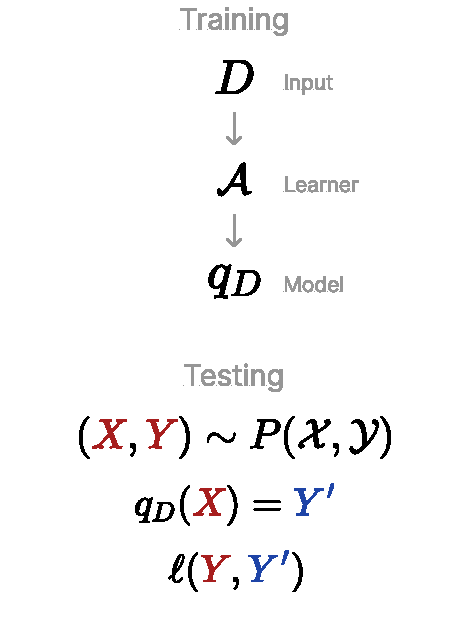
\includegraphics[width=\textwidth]{figma-illustrations/supervised-learning}
	\label{fig:supervised-learning}
	\caption{Illustration of the main components of supervised learning. A learning algorithm $\mathcal{A}$ produces a model $q_D$ given some input $D$. The model is then evaluated on example-outcome pairs of the original data distribution.}
\end{marginfigure}

The desired mapping $q: \mathcal{X} \to \mathcal{Y}$ may be nontrivial such that it is not feasible to come up with explicit rules of how to map examples to outcomes. However, we may try to algorithmically infer such a mapping from a given set of examples and their known outcomes. More specifically, we want to find a deterministic \textit{learning algorithm}, also called \textit{learner}, that, given a random input $D$, produces a mapping $q_D$
\sidenote{
	For the statistical analysis it is essential that the learning algoritm is regarded as deterministic. However, any kind of randomness can be introduced by providing it with random input.
}
.
We call $q_D$ a \textit{model} and note that it is dependent on $D$ .
The task of choosing and configuring a learning algorithm is known as \textit{supervised learning}.

To be useful, a model should not only accurately estimate outcomes for the given training examples, but also provide reasonable predictions for examples that were not part of the input to the learning algorithm. To express this formally in a general setting, we use statistical language.

Consider a probability distribution $P(\mathcal{X}, \mathcal{Y})$ from which realisations of example-training pairs are drawn. We write this as $(X, Y) \sim P(\mathcal{X}, \mathcal{Y})$ where $(X,Y)$ are random variables from a joint distribution.
This distribution is unknown -- else the problem is trivially solved already. In order for our solution to be widely applicable, we strive to make as few assumptions about the distribution $P$ as possible. 

The training dataset $\{ (\vec{x}_{i}, y_{i}) \}_{i=1}^n$ is considered a random vector $D$ drawn from $P(\mathcal{X}, \mathcal{Y})^n$ where $n$ is the number of data points. If there are other sources of randomness in model construction such as, for instance, weight initialisation or neural networks, these can also be considered components of $D$.

\begin{definition}
A \textit{model} is a function $q: \mathcal{X} \to \mathcal{Y}$. In supervised learning with a single model, the model depends on the training input $D$. Its output (prediction) when queried with a random variable $X$ taking values in $\mathcal{X}$ is written as
$$
q_{D}(X)
$$
To shorten notation, we sometimes omit explicitly specifying either random variable, but a dependency on these is always to be understood.
\end{definition}

% \sidenote{
% 	The random variable $D$ can actually encompass various sources of randomness. Most prominently, this is the training data. However, it can also reflect inherent randomness in the learning algorithm. For instance, weights in neural networks are sometimes initialised randomly. Unless otherwise stated, this is the intended meaning. If we explicitly distinguish between training data and model parameters, we denote these with the random variable $\Theta$. We explain this formally in \ref{todo}.
% 	% TODO
% }. 

%
The quality of a single model prediction is measured by means of a \textit{loss function} $\ell: \mathcal{Y} \to \mathcal{Y}$ whose value should be low if the predicted outcome is close to the true outcome. 
To describe the expected loss across the entire distribution, we consider a pair of random variables $(X,Y) \sim P(\mathcal{X}, \mathcal{Y})$. 

\begin{definition} (Risk and Generalisation Error)
The \textit{risk} of a model is the expected loss over all example-outcome pairs.
$$
\text{Risk}(q_{D}) \defeq \mathbb{E}_{(X,Y)\sim P}\left[ \ell(Y, q_{D}(X)) \right] 
$$
%
The quality of a given learning algorithm $\mathcal{A}$ is the expected risk over all possible inputs. We refer to this as the \textit{generalisation error}. 
$$
\text{GE}(\mathcal{A}) \defeq \mathbb{E}_{D}\left[ \text{Risk}(q_{D}) \right]  = \mathbb{E}_{(X,Y), D}\left[ \ell(Y, q_{D}(X)) \right] 
$$
\end{definition}
Note that the choice of the loss function $\ell$ is fundamental to the evaluation of a learning algorithm.

\section{Bias, Variance and their Effects}
 \label{sec:bias-variance-effects}

Since we are ultimately interested in the generalisation error of an ensemble, the question arises what forces influence it. To this end, one can strive to mathematically express the generalisation error in terms of specific meaningful quantities. A classical decomposition is the \textit{bias-variance-decomposition}. 
% Informally, the generalisation error can be decomposed as
% $$
% \text{(error)} = \text{(noise)} + \text{(bias)} + \text{(variance)}
% $$
% The first quantity, \textit{noise} describes inherent noise in the outcomes. It is intrinsic to the given data and can not be influenced by the choice of learner. The second quantity, \textit{bias} is a measure of precision of the learning algorithm \sidenote{Note that we are measuring the \textit{learning algorithm} and not a produced model.}. Intuitively, it describes how precise, on average, a model typically produced by the learning algorithm is. The third quantity, \textit{variance} describes the spread of the learning algorithm. That is, it describes how different the models produced by the learner will be when given different realisations of the input random variable $D$ -- most prominently, different training data sets. 
It is an essential tool to understand learning algorithms in general and ensembles such as Random Forests in particular. For the purpose of this thesis, it is important to understand the decomposition and its motivation in detail. 
We will begin by considering the widely known bias-variance-decomposition for regression using the squared-error loss $\ell(y, y') \defeq (y- y')^2$. We will then proceed to generalise the decomposition to arbitrary loss functions.

\begin{marginfigure} 
  \label{fig:bias-variance-tradeoff}
    \includegraphics[width=\textwidth]{bias-variance/bias_variance_decomposition_with_decision_trees.png}
    \caption{foo!}
    % TODO
\end{marginfigure}

% % TODO bias and variance are measures independent of particular data sample, can use to compare (on same data*set*)

\begin{marginfigure} \label{fig:variance-trees}
    \includegraphics[width=\textwidth]{bias-variance/test_error_of_individual_trees.png}
    \caption{
    Visualising the variance of \textcolor{blue}{Decision Tree} and \textcolor{orange}{Random Forest} models. Each glyph corresponds to the test error of one model trained on a random subset of the full available data. The variation of the test error around the mean test error across many dataset samples is exactly the variance.
    Not only do Random Forests show lower test errors on average, they seem to also have lower variance.
    %  We will explain this observation in \ref{todo}
    % TODO because, in fact, ensemble improvement is solely due to reduction in variance
    %   since var(qbar) = mean(var(qi)) - div/div-eff
    % i.e. the difference between mean tree variances and ensemble variance is exactly the ambiguity/diversity-effect
    }
\end{marginfigure}

% TODO always hyphen, i.e. "squared-error" loss

The variance of a random variable with respect to the squared-error loss is defined as the expected distance in terms of loss to the the expected value.
$$
\Var{X}{X} \defeq \mathbb{E}_{X}\left[ (X - \mathbb{E}_{X}\left[ X \right] )^2 \right]
$$
As such, $\mathbb{E}_{X}\left[ X \right]$ is a centroid to the different realisations of $X$ with respect to the loss function $\ell(Y, Y') = (Y-Y')^2$.
$$
\mathbb{E}_{X}\left[ X \right] = \arg\min _{z} \mathbb{E}_{X}\left[ (X-z)^2 \right] 
$$
Recall that a model is a function dependent on the training input $D$. The variance is a measure of how different the models produced by the learning algorithm will be in terms out outputs if supplied with different realisations of training input $D$.
$$
\Var{D}{q_{D}(X)} = \mathbb{E}_{D}\left[ (q_{D}(X) - \mathbb{E}_{D}\left[ q_{D}(X) \right] )^2 \right] 
$$
$q^\star(X) \defeq \mathbb{E}_{D}\left[ q_{D}(X) \right]$ is the \textit{central model} and does not depend on $D$.

Further, recall that we are considering a joint distribution of example-output pairs $(X,Y)$. We can not assume that the outcomes are not ambiguous. Let $y(X)$ be the outcome associated with $X$.
We measure the variance of actual outcomes $y(X)$ for a given example $X$ around the expected outcome.
$$
\Var{Y}{y(X)} = \mathbb{E}_{Y}\left[ (Y-\mathbb{E}_{Y}\left[ y(X) \right] )^2 \right] 
$$
$y^\star(X) \defeq \mathbb{E}_{Y}\left[ y(X) \right]$ is the \textit{central label} and does not depend on $Y$.

% This is the expected squared error between a random value ($q_{D}$) and the closest non-random value ($\mathbb{E}_{D}\left[q_{D}\right]$). 
% $$
% \Var{D}{q_{D}} \defeq \mathbb{E}_{_{D}}\left[ (q_{D}- \mathbb{E}_{_{D}}\left[ q_{D} \right] )^2 \right]  = \min_{z} \mathbb{E}_{D}\left[ (q_{D} - z)^2 \right] 
% $$
% % TODO #todo already use colours here?
% As such, $\mathbb{E}_{D}\left[ q_{D} \right]$ is a centroid to the different realisations of $q_{D}$ with respect to the loss function $\ell(y,y') = (y-y')^2$.
% This non-random centroid will turn out to be particularly interesting. 
% % For a random variable $Z$, let us denote its centroid with respect to $Y$ as
% % $$
% % Z^\star \defeq \arg \min_{z} \mathbb{E}_Y\left[ (Y - z)^2 \right]
% % $$

% Let's consider two centroids: One with respect to the label distribution and one with respect to the model outputs.
% \begin{itemize}
% \item $y^\star(X) = \arg\min_{z} \mathbb{E}_{Y}\left[ (Y - z(X))^2 \right] = \mathbb{E}_{Y|X}\left[ Y \right]$ is the \textit{expected label} % TODO clarify
% \item $q^\star(X) = \arg \min_{z} \mathbb{E}_{D}\left[ (q_{D}(X) - z(X))^2 \right] = \mathbb{E}_D\left[q_D(X)\right]$ is the \textit{expected model}.
% \end{itemize}

% As such, for the squared-error loss, we can write
% $$
% \Var{q_{D}} = \mathbb{E}_{D}\left[ L(q_{D}, q^\star) \right] 
% $$
Using this notation, the bias-variance decomposition for the squared-error loss is given as follows.
Note that each variance term is the expected distance in terms of loss to a certain centroid.
\begin{align} \label{thm:sqerr-bias-variance-decomp}
\mathbb{E}_{(X,Y), D}\left[ (Y-q_{D}(X))^2 \right]  
% &= 
%   \mathbb{E}_{(X,Y)}\left[ (Y-y^\star(X))^2 \right]  
% + \mathbb{E}_{X, D}\left[ (y^\star(X) - q_{D}(X))^2 \right]  \\
&= \underbrace{\mathbb{E}_{(X,Y)}\left[ (Y-y^\star(X))^2 \right]   }_{\Var{}{Y} ~~ \text{("noise")}} \\
&+ \underbrace{ \mathbb{E}_{X}\left[  (y^\star(X) - q^\star(X))^2\right]  }_{\BiasSq{Y, q} ~~ \text{("learner bias")}} \\
&+ \underbrace{\mathbb{E}_{X, D}\left[ (q^\star(X) - q_{D}(X))^2 \right]   }_{\Var{}{q} ~~ \text{("learner variance")}}
\end{align}
% #todo change BiasSq to just "Bias" -- square is only artifact of squared error
\marginnote{
This decomposition is usually derived by expanding the square \cite{todo}. The cross-terms then vanish due to that $  q^\star = \mathbb{E}_{_{D}}\left[ q_{D} \right]$ and $y^\star = \mathbb{E}_{Y}\left[ y(X) \right]$.
This is but a special case of a more general structure applying to a certain class of losses. We will provide a more general proof in lemmas \ref{thm:bregman-collapse-bias} and \ref{thm:bregman-collapse-variances}.
}

The first term, $\Var{}{Y}$ is independent of $D$ and $q_{D}$. This means we have no means of influencing it with our choice of $q_{D}$.
$\Var{}{Y}$ is also referred to as \textit{noise}, \textit{bayes error} or \textit{irreducible error}. 
The second term, $\Var{}{q}$ measures the variance of our model around its non-random centroid with respect to different realisations of the random training dataset $D$. This can be understood as a measure of spread of the learning algorithm with respect to different realisations of $D$.
The third term, $\BiasSq{q_{D}, Y}$ is the distance in terms of loss between the expected classifier and the expected label. This can be thought of as a measure of precision of the learning algorithm. 

Note that we developed two things:
One the one hand, we derived quantities that measure the notions of bias and variance. On the other hand, by virtue of these quantities appearing in the error decomposition, we have expressed the \textit{effect} these quantities have on the generalisation error.
% This distinction is often overlooked because, like here, for many commonly used losses the quantities and their effects coincide. However, in general this is not necessarily true. 

While the bias-variance decomposition for the squared-error loss is widely accepted, there are many competing decompositions for a range other other loss functions 
\cite{
  kohavi_BiasVarianceDecomposition_,
  hansen_GeneralBiasVariance_2000,
  wood_BiasVarianceDecompositionsMargin_2022,
  didaci_DiversityClassifierEnsembles_2013,
  domingos_UnifiedBiasVarianceDecomposition_,
  pfau_GeneralizedBiasVarianceDecomposition_
  }. For instance, we are particularly interested in the \zeroone-loss for classification. A decomposition of it where the model variance is independent of the outcome variable as in term \ref{eq:variance-term} is been proven to not exist \cite{wood_UnifiedTheoryDiversity_2023}. We will now argue that approaching the matter from the perspective of such \textit{loss-effects} allows us to state a general bias-variance decomposition that holds for any loss function. The decomposition for the squared-error loss is a special case of it.

\marginnote{
  Note that the arguments of loss-effect appear in inverse order in the difference. This is to give the expression a suggestive shape since in section \ref{sec:bregman-divergences}, we will show that, for a Bregman divergence $B_\phi$, it holds that
  $$
  \mathbb{E}\left[\LE{Z'}{Z}\right] = \Breg{Z'}{Z}
  % TODO check order of arguments
  $$
}
\begin{definition} (Loss-Effect) For a loss functon $\ell$, and random variables $Y, Z, Z'$, we define the change in loss between $Z$ and $Z'$ in relation to $Y$ as:
  $$
  \LE{Z}{Z'} \defeq \ell(Y, Z') - \ell(Y, Z)
  $$
  \label{def:loss-effect}
\end{definition}

\begin{definition}
\label{def:central-model}
(Central model) Given a model $q$, it's central model is the centroid with respect to $D$:
$$
q^\star \defeq \arg\\min_{z} \mathbb{E}_{D}\left[ \ell(z, q_{D}) \right] 
$$
\end{definition}

\begin{definition}
\label{def:central-label}
(Central label) The central label is 
$$
y^\star \defeq \mathbb{E}_{Y|X}\left[ Y \right] 
$$
\end{definition}

The \textit{variance-effect} is the expected change in loss caused by using $q_{D}$ instead of the non-random centroid $q^\star(X)$. Likewise, the \textit{bias-effect} is the expected change in loss caused by using the expected model instead of the expected label. In the following, to lighten notation, we will omit explicitly stating the dependence on $X$.
\sidenote{In the original publication \cite{james_GeneralizationsBiasVariance_}, bias-effect is called the \textit{systematic effect}, i.e. the effect of the systematic components. However, it is clearer to call this \textit{bias-effect}, particularly when we begin to introduce notions of diversity in \ref{sec:diversity-measures}.}
Formally:
\begin{align*}
\text{Bias-Effect} &\defeq \mathbb{E}_{D,Y}\left[ \ell(Y, q^\star) - \ell(Y, y^\star) \right] \\
\text{Variance-Effect} &\defeq \mathbb{E}_{D,Y}\left[ \ell(Y, q_{D}) - \ell(Y, q^\star) \right] 
\end{align*}


\begin{marginfigure}
  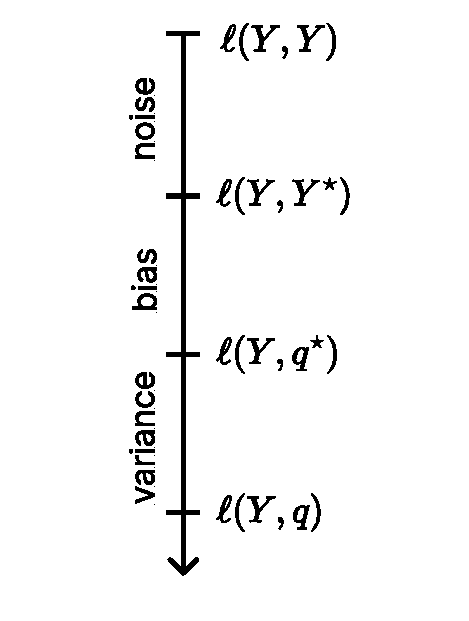
\includegraphics[width=\textwidth]{figma-illustrations/effect-decomp.pdf}
  \caption{
    Illustration how the bias-variance-effect decomposition decomposes the loss $\ell(Y, q)$ into meaningful segments.
  }
  \label{fig:margin-decomp-geometry}
\end{marginfigure}

This allows us to state a decomposition of the generalisation error simply in terms of loss-effects.
$$
\mathbb{E}_{}\left[ \ell(Y,q) \right]  = \mathbb{E}_{}\left[  \underbrace{ \ell(Y, y^\star) }_{\text{"noise"} }
+
\underbrace{ \ell(Y, q^\star) - \ell(Y, y^\star) }_{\text{"bias-effect"} }
+ 
\underbrace{ \ell(Y, q) - \ell(Y, q^\star) }_{\text{"variance-effect"} } \right]
$$
Note that the individual terms on the right-hand side simply cancel out and reduce to $\ell(Y, q)$. As illustrated in figure \ref{fig:margin-decomp-geometry}, this decomposition divides the the interval from $\ell(Y, Y) = 0$ to $\ell(Y, q)$ into meaningful sections. 
Note that this decomposition depends solely on the linearity of expectation and is independent of the loss function $\ell$ or the definitions of $y^\star$ and $q^\star$.

For the squared-error loss $\ell(Z, Z') = (Z - Z')^2$, bias-effect equals bias and variance-effect equals variance.
$$
 \mathbb{E}_{}\left[ \ell(Y, q^\star) - \ell(Y, y^\star) \right]  = \mathbb{E}_{}\left[ \ell(y^\star, q^\star) \right]
$$
$$
 \mathbb{E}_{}\left[ \ell(Y,q) - \ell(Y, q^\star) \right]  = \mathbb{E}_{}\left[ \ell(q^\star, q)  \right] 
$$
Thus, the bias-variance decomposition for the squared-error loss is a special case of this.

\marginnote{
  Note that while for the squared error the variance compares \textit{model predictions}, the variance-effect is based solely on the \textit{change in loss}. In section \ref{sec:bregman-divergences}, we will see that the former is in fact only a special property of a specific family of loss functions.
% TODO see e.g. arguments on "variance" reduction
}
\begin{theorem} (Bias-Variance-Effect-Decomposition \cite{james_GeneralizationsBiasVariance_})
\label{thm:bias-variance-effect}
For any loss function $L$, it holds that
\begin{align*}
\mathbb{E}_{(X,Y), D}\left[ \ell(Y, q_{D}) \right]  
&= 
\underbrace{\mathbb{E}_{(X,Y)}\left[ \ell(Y, y^\star) \right]  }_{\text{noise}}
+ \underbrace{\mathbb{E}_{X)}\left[ \LE{q^\star, y^\star} \right] }_{\text{bias-effect}}
+ \underbrace{\mathbb{E}_{X,D}\left[ \LE{q_D, q^\star} \right] }_{\text{variance-effect}}  \\
% \\ 
% \text{for} \hspace{1em}
% & \LE{q^\star}{y^\star} = \ell(Y, q^\star) - \ell(Y, y^\star) \\ \\
% &\LE{q^\star}{q_D} = \ell(Y, q_{D}) - \ell(Y, q^\star)
\end{align*}
\end{theorem}
This decomposition holds for \textit{any} loss function since, by linearity of expectation, the individual terms on the right-hand-side simply cancel out. Further, this decomposition is independent of the definitions of $y^\star$ and $q^\star$.






\section{Bregman Divergences and Centroids}

To measure the difference between predicted and ground-truth outcomes, we use a loss function $\ell$. The choice of loss function depends on the data domain, the learning task and computational considerations. 

Often, learners are analysed with respect to a specific loss function, such as the squared-error loss \cite{scornet_ConsistencyRandomForests_2015} for regression or the \zeroone-loss \cite{theisen_WhenAreEnsembles_2023} or the KL-divergence \cite{webb_EnsembleNotEnsemble_2019} for classification. The well-known bias-variance decomposition for the squared-error loss is usually shown directly in teaching materials \cite{tibshirani_ElementsStatisticalLearning_2017, weinberger_Lecture12Bias_}. The question then arises which properties are specific to the loss function and which are part of a more general structure.

We will now define a family of loss functions, called \textit{Bregman divergences}, that encompasses many widely used loss functions in supervised learning (see table \ref{tab:bregman-examples}). 
% We are interested in when and how one can improve the generalisation error by combining multiple models into an ensemble. We will consider generally for arbitrary loss functions, and then identify Bregman divergences of an important special case.

\begin{marginfigure} \label{fig:bregman-div-intuition}
    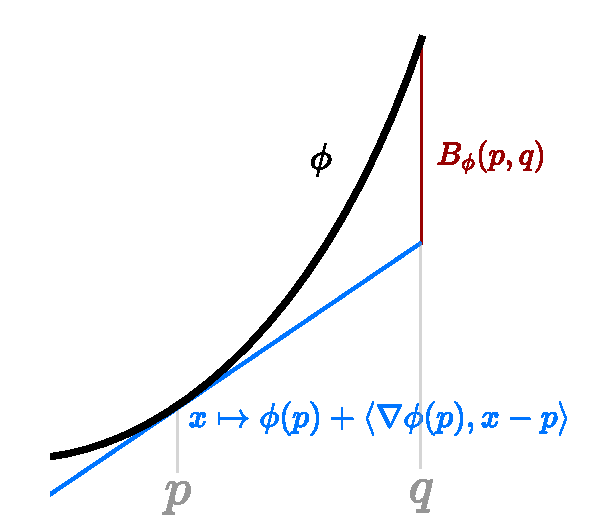
\includegraphics[width=\textwidth]{figma-illustrations/bregman-div-intuition}
    \caption{Given a strictly convex generator $\phi$, the Bregman divergence for points $p, q$ is the difference between the linear approximation around $p$ and $\phi$ at the point $q$. }
\end{marginfigure}
% TODO never pagebreak in theorem/definition boxes
\begin{definition} \label{def:bregman-divergence}
\textit{(Bregman Divergence \cite{pfau, adlam22})} The Bregman divergence $\Breg{p}{q} : \mathcal{S} \times \mathcal{S}\to \mathbb{R}$ is defined based on a generator function $\phi$ as follows:
$$
\Breg{p}{q} \defeq \phi(\vec{p}) - \phi(\vec{q}) - \inner{\nabla \phi(q)}{(\vec{p} - \vec{q})}
$$
where $\inner{\cdot}{\cdot}$ is the inner product, $\nabla \phi(\vec{q})$ is the gradient vector of $\phi$ at $\vec{q}$ and $\phi: \mathcal{S} \to \mathbb{R}$ is a strictly convex function on a convex set $\mathcal{S} \subseteq \mathbb{R}^k$ such that it is differentiable on the relative interior of $\mathcal{\S{}}$.
\end{definition}


\begin{table*}[hb]
    \centering
    \caption{
      Examples of commonly used loss functions that are Bregman divergences 
      \cite{banerjee_ClusteringBregmanDivergences_2004, wood_UnifiedTheoryDiversity_2023} 
    }
    % TODO formatting of table
    \begin{tabular}{|l|l|l|l|}
    \hline
        Divergence $\Breg{p}{q}$ & Generator $\phi(q)$ & Domain $S$ & Loss function \\ \hline
        $(p-q)^2$ & $q^2$ & $\mathbb{R}$ & Squared Error \\ \hline
        $x \log \left(\frac{x}{y}\right)+(1-x) \log \left(\frac{1-x}{1-y}\right)$ & $x \log x+(1-x) \log (1-x)$ & $[0,1]$ & Logistic loss \\ \hline
        $\frac{x}{y}-\log \left(\frac{x}{y}\right)-1$ & $-\log x$ & $\mathbb{R}_{>0}$ & Ikura-Saito distance \\ \hline
        $\mid\mid x-y \mid\mid^2$ & $\mid\mid x\mid\mid^2$ & $\mathbb{R}^d$ & Squared Euclidean distance \\ \hline
        $(x-y)^\top A (x-y)$ & $x^\top A y$ & $\mathbb{R}^d$ & Mahalanobis distance \\ \hline
        $\sum_{j=1}^d x_j \log _2\left(\frac{x_j}{y_j}\right)$ & $\sum_{j=1}^d x_j \log _2 x_j$ & $d$-simplex & KL-divergence \\ \hline
        $\sum_{j=1}^d x_j \log \left(\frac{x_j}{y_j}\right)-\sum_{j=1}^d\left(x_j-y_j\right)$ & $\sum_{j=1}^d x_j \log x_j$ & $\mathbb{R}^d_{\geq {0}}$ & Generalized I-divergence \\ \hline
        $\sum_{j=1}^d x_j \log x_j$ & $\sum_{j=1}^d x_j \log x_j$ & $\mathbb{R}_{\geq {0}}$ & Poisson loss \\ \hline
    % TODO maybe add gini imp here
    \end{tabular}
    \label{tab:bregman-examples}
\end{table*}

% \marginfigfromsource{fig:bregman-intuition-1d}{symlinks/illustrations/bregman/bregman-intuition-1d-ikura-saito}

% Recall that in \ref{sec:bias-variance-effects}, we have considered centroids with respect to the squared error, which is symmetric. 
% Bregman divergences are in general not symmetric and hence we need to define \textit{left} and \textit{right} centroids.
% TODO relate centroids to bregman information etc in banerjee_ClusteringBregmanDivergences_2004

% TODO repeating a bit here, maybe remove first few paragraphs
% The "statistical" variance $(X - \mathbb{E} \left[ X \right])^2$ is the expected distance around the centroid as measured by the squared-error loss. Other loss functions imply different notions of variance.
%
% A common measure is the "statistical" variance $(X - \mathbb{E} \left[ X \right])^2$. One can see that $\mathbb{E}_{}\left[ X \right]$ is in fact the minimizer of the expected squared distances to realisations of $X$:
% $$
% \mathbb{E}_{}\left[ X \right]  = \arg\min_{z} \mathbb{E}_{X}\left[ (X - z)^2 \right] 
% $$
% As such, $\mathbb{E}_{}\left[ X \right]$ is a \textit{centroid} of the realisations of $X$ with respect to the squared error. 
%
% This variance of a random variable around its centroid will be a very basic building block in our analysis of the generalisation error of ensembles. Concretely, we will explain that, except for the bias term, the well-known bias-variance decomposition in fact considers only such variances:
% \begin{itemize}
% \item The variance of the label around the expected label -- this commonly referred to as \textit{label noise} or \textit{irreducible noise}.
% \item The variance of a concrete model $q_{D}$ trained on a dataset $D$ around the expected model -- this is commonly referred to as the \textit{(learner) variance}.
% \end{itemize}
% Further, we will proceed to show that a crucial component to ensemble learning will be the variance of a learner parameterised by $\Theta$ around its expected model with respect to the distribution of $\Theta$.
% We will see that all these quantities can indeed be expressed as variances due to a specific property of Bregman divergences. For the \zeroone-loss, this takes a different form.
% TODO somewhere else: this means that bias-variance-covariance decomposition is an artifact of squared error (pullling out the covariance, I think) -- although expressing in terms of disagreement is still possible, cf bounds by theisen.
%
In order to talk about variances with respect to Bregman divergences, we need a notion of a centroid with respect to a Bregman divergence. Bregman divergences are in general not symmetric and hence there is a \textit{left} and \textit{right} centroid.

\begin{lemma} (Left and right Bregman centroids, \cite{pfau_GeneralizedBiasVarianceDecomposition_})
  \label{thm:bregman-centroids}
    Let $B_{\phi}$ be a Bregman divergence of generator $\phi: \mathcal{S} \to \mathbb{R}$. For a random variable $Y$ taking values in $\mathcal{S}$, it holds that
\begin{itemize}
    \item the \textit{right Bregman centroid} is $$\arg \min_z \mathbb{E}_{X}\left[ \Breg{X}{z}  \right] = \mathbb{E}_{}\left[ X \right]$$
    \item the \textit{left Bregman centroid} is $$\arg\min_{z}  \mathbb{E}_{X}\left[ \Breg{z}{X}\right] = (\nabla \phi)^{-1} \mathbb{E}_{}\left[ \nabla \phi(X) \right] \defeq \mathcal{E}\left[X\right]$$
\end{itemize}
  If $B_\phi$ is symmetric, i.e. $\Breg{Y}{Y'} = \Breg{Y'}{Y}$ then $\mathbb{E}\left[X\right] = \mathcal{E}\left[X\right]$.
\end{lemma}
\begin{definition} (Dual expectation \cite{pfau_GeneralizedBiasVarianceDecomposition_})
  \label{def:dual-expectation}
  The left Bregman centroid is the expected value in the dual space implied by $\nabla\phi$. Due to this, we define the dual expectation as  
  $$\mathcal{E}\left[X\right] \defeq (\nabla \phi)^{-1}\mathbb{E}_{}\left[ \nabla \phi(X) \right]$$ 
\end{definition}

% The left Bregman centroid will be important for considering the variance of a learner around its parametrisation $\Theta$.
% TODO a visual here

A generalised measure of variance is then the expected divergence around a Bregman centroid.

\begin{definition}
	\label{def:bregman-information}
	The variance around the right Bregman centroid is known as the 
	\textit{Bregman information} 
  $I_{\phi}(X)$
  \cite{banerjee_ClusteringBregmanDivergences_2004}.
$$
I_{\phi}(X) \defeq \mathbb{E}_{X}\left[ \Breg{X}{\mathbb{E}_X\left[ X \right] } \right] 
$$
\end{definition}
% TODO so decision tree split point search is basically 2-means?!

In other words, the choice of loss function implies a measure of variance. Various well-known variance measures can now be seen to actually be implied by a Bregman divergence.
For example, let $X = \{ X_{1}, \dots, X_{n} \} \subset \mathbb{R}^d$. Then the squared Euclidean distance corresponds to the \textit{sample variance} \cite{banerjee_ClusteringBregmanDivergences_2004}.
$$
\Breg{p}{q} =~\mid\mid p-q\mid\mid^2 ~ ~ \rightarrow ~ ~ 
I_{\phi}(X) = \frac{1}{n} \sum_{i=1}^n (X_{i} - \mathbb{E}_{}\left[ X \right] )^2
$$
For the KL-divergence, the Bregman information is the \textit{mutual information}. Consider a random variable $X$ over probability distributions with probability measure $p$ \cite{banerjee_ClusteringBregmanDivergences_2004}.
$$
\Breg{u}{v} = \sum_{j=1}^d u_{j} \log \left( \frac{u_{j}}{v_{j}} \right) 
~ ~ \rightarrow ~ ~  I_{\phi}(X) = 
\sum_{i=1}^n \sum_{j=1}^m p\left(u_i, v_j\right) \log \frac{p\left(u_i, v_j\right)}{p\left(u_i\right) p\left(v_j\right)}
$$
% TODO entropy and log-loss
% see https://chat.openai.com/c/26e594d3-91f1-4bec-9f9a-8cb866ede63a
% (can give this as starred proof)

% TODO properly, generally define q^star -- should be dual expectation! (also in case of effect-decomp?)
% TODO diversity is upper-bounded by *average* variance (not just ensemble variance) (as consequence of qstar lemma in homogeneous)





\chapter{Ensemble Learning}
\label{chapter:ensemble-learning}

\textit{Ensemble Learning} is the method of training $M$ individual models $q_{1}, \dots, q_{M}$ for a given task and aggregating their output via an \textit{ensemble combiner} $\bar{q}$ to form an ensemble prediction \cite{zhou_EnsembleMethodsFoundations_2012}.
The individual models $q_{1}, \dots, q_{M}$ are referred to as \textit{members}. When all members are constructed using the same learning algorithm, we call it a \textit{homogeneous} ensemble. The learning algorithm is then referred to as the \textit{base learner}. Otherwise the ensemble is \textit{heterogeneous}. 
% When analysing the generalisation error, we refer to $\bar{q}$ as the \textit{ensemble model}. When considering how to actually combine ensemble predictions, we also refer to $\bar{q}$ as the \textit{combiner}. 


\section{Methods}
\label{sec:ensemble-learning-methods}
There are three main variants of ensemble learning \cite{mienye_SurveyEnsembleLearning_2022}:
\begin{itemize}
\item \textit{Parallel}: All members are trained independently. The outputs of all members are then aggregated to form the ensemble prediction.
\item \textit{Stacking} or \textit{Meta-Learning}: All members are trained independently. The member outputs serve as input data for another learning algorithm, which then provides the ensemble prediction.
\item \textit{Sequential}: Members are trained in sequence. The output of the previous ensemble member informs the construction of the next member.
\end{itemize}
% TODO diagrams
Random Forests \cite{breiman_RandomForests_2001} are an example of parallel ensemble construction. $M$ decision trees are constructed independently and the tree's predictions are aggregated by a kind of mean (see section \ref{sec:decision-trees}). A classical example for sequential ensemble construction is \textit{Boosting} \cite{schapire_BoostingFoundationsAlgorithms_2012}. In boosting algorithms, the ensemble combiner $\bar{q}$ is not a mean but a (weighted) sum $\bar{q} = \sum_{i=1}^M \alpha_{i}q_{i}$. The first member $q_{1}$ provides a base prediction. Successive members are then trained to predict not an output value but \textit{increments} (\textit{pseudo-targets}) to the base prediction such that the sum $\alpha_{1}q_{1} + \alpha_{2}q_{2} + \dots$ moves towards a more precise prediction. 
In this thesis, we will focus on the Random Forest learner and variations of it. 
% TODO reintroduce if we get to actually putting that down
% Although it can be seen as a parallel ensemble construction method, we will see that it can also be understood as a boosting algorithm (see \ref{todo}).


\section{Applications}

% https://www.maths.usyd.edu.au/u/pengyi/publication/EnsembleBioinformatics-v6.pdf
% from there:
% - https://www.pnas.org/doi/full/10.1073/pnas.0709868104
% - https://www.pnas.org/doi/full/10.1073/pnas.0230559100

\section{Notation}
\label{sec:ensemble-learning-notation}
% TODO somewhere, prefix that combiner is rather ad-hoc, arithmetic mean, but can see that dual expectation actually makes sense

In the supervised learning setting with a single model, we have defined the model as a function $q_{D}(X)$. In ensemble learning, $M$ individual models are constructed and their outputs are aggregated via an ensemble combiner $\bar{q}$ to form an ensemble output. The individual models are referred to as \textit{members}. 

\begin{marginfigure}
  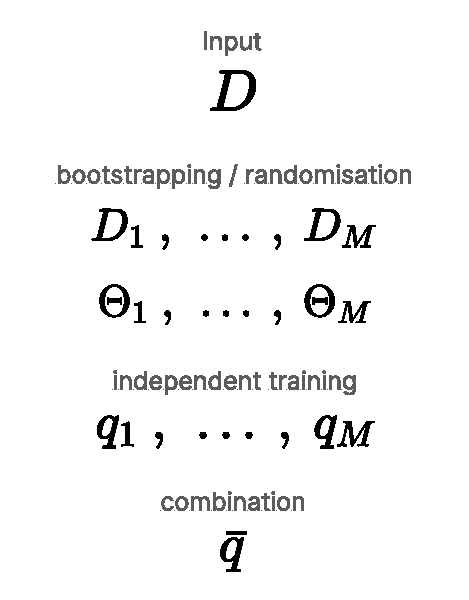
\includegraphics[width=\textwidth]{figma-illustrations/ensemble-learning.pdf}
  \caption{
    Illustration of parallel ensemble learning.
  }
\end{marginfigure}
Analysing ensembles means analysing differences between the members. There are two dimensions in which ensemble members can differ. First, in terms of provided training data. 
\sidenote{For instance, each learner may be trained on a random subset of the available training data (see section \ref{sec:random-forest-scheme})}
Second, in terms of other randomness used in model construction.
\sidenote{For instance, random numbers used in decision tree construction (see section \ref{sec:decision-trees}).}
To distinguish these two sources, we sometimes denote the training data as a random vector $D = (D_{1}, \dots, D_{M})$ and other parameters as $\Theta = (\Theta_{1}, \dots, \Theta_{M})$. 
\begin{definition} (Ensemble member model) The $i$-th ensemble member model $q_{i}: \mathcal{X} \to \mathcal{Y}$ is a function depending on training input $D_{i}$ and additional parameters $\Theta_{i}$.
$$
q_{D_{i}, \Theta_{i}}(X)
$$
To shorten notation, we also write $q_{i} \defeq  q_{D_{i}, \Theta_{i}}(X)$.
\end{definition}
Due to that the $i$-th member then depends only on $D_{i}$ and $\Theta_{i}$ and is independent of $D_{j}$ and $\Theta_{j}$ for $j \not= i$, using the law of total expectation (see lemma \ref{thm:law-of-total-expectation}), we can write
$$
\mathbb{E}_{D}\left[ q_{i} \right] = \mathbb{E}_{D_{j \not= i}}\left[ \mathbb{E}_{D_{i}}\left[ q_{i} \right]   \right]  = \mathbb{E}_{D_{i}}\left[ q_{i} \right] 
$$
and likewise for $\Theta$. 



The output of an ensemble is produced by aggregating the outputs of the member models using a combiner function. 
\marginnote{
  For the \zeroone-loss for a $k$-class classification problem, the implied combiner is the plurality vote:
  $$
  \bar{q} = \arg\min_{z \in [k]} \mathbb{E}_{\Theta}\left[ \Lzo{z}{q_{\Theta}} \right]  
  $$
  For Bregman divergences, i.e. $\ell = B_\phi$, the combiner implied by $\ell$ is the dual expectation:
  \begin{align*}
  \bar{q} &= \mathcal{E}_{\Theta}\left[ q_{\Theta, D} \right] \\
  &= (\nabla \phi)^{-1} \mathbb{E}_\Theta \left[\nabla \phi (q_\Theta)\right]
  \end{align*}
  The squared-error loss is a symmetric Bregman divergence and hence the ensemble combiner is the arithmetic mean:
  \begin{align*}
    \bar{q} &= \mathcal{E}_\Theta \left[X\right] = \mathbb{E}_\Theta \left[X\right] \approx \Mavg q_i
  \end{align*}
}
\begin{definition}
   \label{def:ensemble-combiner}
   (Ensemble combiner) The ensemble combiner $\bar{q} : \mathcal{X} \to \mathcal{Y}$ for a given loss function $\ell$ is the centroid with respect to model parameters $\Theta$: 
% TODO would sort of need to motivate that we already use dual exp here
$$
\bar{q} \defeq \arg\min_z \mathbb{E}_\Theta \left[ \ell(z, q_\Theta) \right]
$$
\end{definition}
Note that this is the central model with respect to $\Theta$ (compare definition \ref{def:central-model}).
For Bregman divergences, this shows to be the dual expectation (def. \ref{def:dual-expectation}). This definition agrees with combiners commonly used in practise (plurality vote, arithmetic mean). It links combiners to loss functions. Further, it suggests combiners for other loss functions. In each case, using a combiner as defined here enables a very general and expressive theory of ensemble diversity and a decomposition of the ensemble generalisation error exactly measuring ensemble improvement due to diversity.

An ensemble is homogeneous iff $\Theta_{1}, \dots, \Theta_{M}$ are identically and independently distributed. This is the case if the member models are constructed according to the same base learner and do not influence each other. 

\begin{lemma}
 \label{thm:qstars-same} 
  $\star$ In homogeneous ensembles, the central models of any two members and the combiner are the same. That is, for any $i, j \in \{ 1, \dots, M \}$ it holds that
$$
q_{i}^\star = q_{j}^\star = \bar{q}^\star
$$
\end{lemma}
\begin{proof}
If $D_{1}, \dots, D_{M}$ and $\Theta_{1}, \dots, \Theta_{M}$ are identically distributed and independent, it holds that
$$
q_{i}^\star = \mathbb{E}_{D}\left[ q_{D_{i}, \Theta_{i}} \right]  = \mathbb{E}_{D_{i}}\left[ q_{D_{i}, \Theta_{i}} \right]  
= \mathbb{E}_{D_{j}}\left[ q_{D_{j}, \Theta_{i}} \right] = q_{j}^\star
$$

% TODO verify that in cases such as sqerr, nabla phi = id??
For the ensemble combiner, it holds that
\begin{align*}
\bar{q}^\star &= \mathcal{E}_{\Theta}\left[ q_{D,\Theta} \right] ^\star = \mathcal{E}_{D}\left[ \mathcal{E}_{\Theta}\left[ q_{D,\Theta} \right]   \right] \\
&= (\nabla \phi)^{-1} \mathbb{E}_{D}\left[ (\nabla \phi) (\nabla \phi)^{-1} \mathbb{E}_{\Theta}\left[ q_{D,\Theta} \right]   \right] \\
&= \mathcal{E}_{\Theta}\left[ \mathcal{E}_{D}\left[ q_{D, \Theta} \right]  \right] = \mathcal{E}_{\Theta}\left[ q_{\Theta}^\star \right] 
\end{align*}
Due to the result above, $q_{\Theta}^\star$ is constant over $\Theta$ and thus $\mathcal{E}_{\Theta}\left[ q_{\Theta}^\star \right] = q_{\Theta}^\star$.

Both properties also hold for dual expectations for Bregman divergences defined in definition \ref{thm:bregman-centroids}.
\end{proof}

A basic measure for classification ensembles under the \zeroone-loss is the winning margin of the majority vote.
% TODO resolve ambiguous terms majority/plurality
\begin{definition} (Ensemble margins for majority voting \cite{breiman_RandomForests_2001})
The margin for class $y$ of an example $x$ is the difference between the number of member votes for class $Y$ and the number of votes for the next-best class.
	$$
\mr(x,y) \defeq \Mavg \ind{q_{i} = y} - \max_{j \neq y} \Mavg \ind{q_{i} = j} \in [-1, 1]
$$
% TODO maybe express with expectations instead
\label{def:ensemble-margin}
\end{definition}

% TODO not sure if we'll ever need this
If ensemble members are parameterised by $\Theta$, from the statistical point of view, we can also write
$$
\mr(x,y) = \prob{\Theta}{q_{\Theta} = y} - \max_{j \not=y} \prob{\Theta}{q=j}
$$
where the probabilities are conditioned on $x$. For binary classification under the \zeroone-loss, the ensemble margin is linearly related to the ratio of incorrect members $\Mavg \Lzo{y}{q_{i}(x)} \approx \prob{\Theta}{q \not= y}$.
$$
\begin{align*}
\mr(x,y) &= \prob{\Theta}{q=y}  - \prob{\Theta}{q \not= y} \\
&= (1 - \prob{\Theta}{q \not= y}) - \prob{\Theta}{q \not= y} \\
&= 1 - 2 \prob{\Theta}{q \not= y}
\end{align*}
$$
So, $\mr(x,y) = 1 - 2 \Mavg\Lzo{y}{q_{i}(x)}$.


% When considering an actual ensemble of trained models, we understand $\bar{q}$ and $q_{1}, \dots, q_{M}$ to be functions $\mathcal{X} \to \mathcal{Y}$. In the statistical setting, $\bar{q}, q_{1}, \dots, q_{M}$ are random variables dependent on a random variable $X$ that represents the query example. Further, combiner and members depend on the input $D$ to the ensemble construction algorithm. For sake of brevity, this dependence is implicit in the notation and we write $q_{i} \defeq q_{i}(X;D)$.

% In the original supervised learning setup (see section \ref{sec:supervised-learning}), we considered $D$ to be the random input to the learning algorithm. This usually includes a training dataset (which is assumed to be randomly sampled from an underlying distribution). Further, this can include any kind of randomness used by the algorithm.
% In ensemble learning, we are considering multiple learning algorithms. Each of these individual learners receives its own input. For instance, each learner may be trained on a random subset of the available training data (see section \ref{sec:bootstrapping}). To this end, we consider $D$ to be a random vector of random variables $(D_{1}, \dots, D_{M})$. 
% Due to the law of total expectation, it holds that
% $$
% \mathbb{E}_{D}\left[ \ell(y, q(x; D_{i})) \right]  = \mathbb{E}_{D_{i}}\left[ \ell(y, q(x; D_{i})) \right] 
% $$
% even if there are dependencies between the components of $D$. This means that for an individual member $q_{i}$, an expectation over $D$ reduces to an expectation over $D_{i}$. This justifies considering expectations over $D$ in general.

% In some cases, it is clearer to distinguish between input training data and other random parametrisation of the individual learner. In this case, we take $D$ to be the training data and $\Theta$ to be a random variable representing other parameters. 
% One can then write $\bar{q} = \mathbb{E}\left[q(x; \Theta)\right]$.
% TODO not sure whether that's correct -- shouldnt this be the dual expectation?


% Ultimately, we are interested in the generalisation error of the ensemble given by $\mathbb{E}_{(X,Y),D}\left[ \ell(Y, \bar{q}_{D}(X)) \right]$ where the subscript indicates that the ensemble model depends on the random variable $D$. Since $\bar{q}$ is produced by aggregating the member outputs $q_{1}, \dots, q_{M}$ the essential question is how the member models have to behave in order for ensemble techniques to be effective. 


% special cases for binary classification, relate to ratio of incorrect members / examples
% TODO -- as such, really close to other decomps

% Let
% $$
% \hat{j} = \hat{j}(\vec{X}, Y) = arg\max_{j\neq Y} \prob{\Theta}{q_{\Theta} = j}
% $$
% denote the next-best vote. So, using the elementary "probability is expectation of indicator" trick:
% \begin{align}
% \mr(\vec{X}, Y)  &= \prob{\theta}{q_{\Theta} = Y} - \prob{\Theta}{q_{\theta} = \hat{j}} \\
% &= \mathbb{E}_{\Theta}\left[ \ind{q_{\Theta} =Y } - \ind{q_{\Theta} = \hat{j}} \right] 
% \end{align}
% Def **Raw margin function** $\rmg(\Theta, \vec{X}, Y)$: Define
% $$
% \rmg(\Theta, \vec{X}, Y) := \ind{q_{\theta} = Y} - \ind{q_{\theta} = \hat{j}}
% $$
% ...such that the RF margin function is the expectation of the raw margin function with respect to $\Theta$:
% $$
% \mr(\vec{X}, Y) = \mathbb{E}_{\Theta}\left[  \rmg(\Theta, \vec{X}, Y)  \right] 
% $$


\section{Motivation}
\label{sec:ensemble-learning-motivation}

We will now review some classical arguments that motivate ensemble learning. We do this to provide context to the results in chapter \ref{sec:diversity}, which also show when and how ensemble learning is beneficial.

\paragraph{Ensemble improvement is non-negative} The arithmetic mean combiner can be seen as approximating an expectation over member models, i.e. $\bar{q} = \mathbb{E}_{\Theta} \left[q_{\Theta}\right] \approx \Mavg q_i$.
This motivated \cite{abe_PathologiesPredictiveDiversity_2023} to invoke Jensen's inequality
\marginnote{Jensen's inequality, in a probabilistic setting, states that, for a function $\phi:\mathbb{R} \to \mathbb{R}$ and a random variable $X$
$$
\phi \text{~convex} \rightarrow \phi\left(\mathbb{E}_{}\left[ X \right] \right) \leq \mathbb{E}_{}\left[ \phi(X) \right] 
$$
}
. For a loss function $\ell$ that is convex in its first argument, it holds that
$$
\underbrace{
\ell(Y, \mathbb{E}_{\Theta}\left[ q_{\Theta}(X)\right] ) 
}_{\text{"ensemble loss"}}
~ ~ \leq ~ ~ 
\mathbb{E}_{\Theta}\left[ 
\underbrace{
\ell(q_{\Theta}(X), Y)  
}_{\text{"member loss"}}
\right]
$$
and thus
$$
\mathbb{E}_{{\Theta}}\left[ \ell (q_{\Theta}(X),Y) \right]  -
\ell(\mathbb{E}_{\Theta}\left[ q_{\Theta}(X) \right] ,Y ) \geq 0
$$
\begin{corollary}
  For convex loss functions and using the arithmetic mean combiner, ensembling can never hurt performance: The ensemble loss is always smaller-equal than the average member error.
\end{corollary}
% This shows that, for convex loss functions and the arithmetic mean combiner, the ensemble loss is always smaller-equal than the average member error.
\cite{abe_PathologiesPredictiveDiversity_2023} interpret the difference between these quantities, as a measure of ensemble improvement. 

\paragraph{Ensemble bias equals average member bias}
It can be shown that the bias of a homogeneous ensemble is equal to the average bias of the ensemble members. We will give an illustrative argument for the arithmetic mean combiner here.
We will show this in detail in a more general and inuitive way in chapter \ref{sec:diversity}.

\begin{lemma} (Ensemble bias equals average member bias under arithmetic mean combiner \cite{louppe_UnderstandingRandomForests_2015})
  \label{thm:ensemble-bias-equals-average-bias}
$$
\mathbb{E}_{X}\left[ \ell(y^\star(X), \bar{q}^\star(X)) \right] 
= \mathbb{E}_{X}\left[ \ell(y^\star(X), q^\star(X)) \right] 
% TODO also need exp over D
$$
\end{lemma}
\begin{proof}
Consider individual learner inputs $D = (D_{1}, \dots, D_{M})$. Each member depends on some $D_{i}$ and the combiner $\bar{q}$ depends only on $D$. Assuming that $D_{1}, \dots, D_{M}$ are independent and identically distributed, we can write
$$
\mathbb{E}_{D, \Theta}\left[ \bar{q} \right] = \mathbb{E}_{D}\left[ \Mavg q_{D_{i}} \right] = \Mavg \mathbb{E}_{D_{i}}\left[ q_{D_{i}} \right] = \mathbb{E}_{D'}\left[ q_{D'} \right]
$$
where $D'$ is distributed as any $D_{i}$. We can conclude $\mathbb{E}_{D}\left[ \bar{q} \right] = \mathbb{E}_{D}\left[ q_{D} \right]$ (see section \ref{sec:ensemble-learning-notation}).
This implies
% TODO pull this out into lemma, also using this somewhere else
% need to reorder a bit anyway, havent even introduced star notation yet
% TODO recap/ref definition of q^star
$$
\bar{q}^\star = \mathbb{E}_{D}\left[ \bar{q} \right]  = \mathbb{E}_{D}\left[ q_{D} \right]  = q^\star
$$
and thus the bias of the ensemble is the same as the bias of a member model $q$.
\end{proof}
This argument depends on the linearity of expectations, the arithmetic mean combiner and the fact that the ensemble is homogeneous. We will later show this more directly for any loss function and any combiner (see \ref{sec:unchanged-bias}).

\begin{corollary}
For homogeneous ensembles under the arithmetic mean combiner, ensemble improvement is solely due to variance reduction.
% TODO clarify! what is ensemble improvement?
\end{corollary}
% TODO and later see that variance reduction is exactly measured by diversity -- summarise that clearly somewhere -- maybe even put it in a theorem
% really in this thesis, we're the first to provide a comprehensive picture onto all this from the lens of the diversity decomp



\paragraph{Variance reduction for squared-error regression} 
Consider the regression setting under the squared-error loss and the arithmetic mean combiner.
Assume $q_{1}, \dots, q_{M}$ are identically and independently distributed with equal variance $\sigma^2$.
$$
	\Var{}{\bar{q}} = \Var{}{\Mavg q_{i}} = \frac{1}{M^2} \sum_{i=1}^M \Var{}{q_{i}} = \frac{1}{M} \sigma^2
$$
As the number of members $M$ increases, the ensemble variance is reduced. Further, one can also see that the interactions between members determine the variance reduction. Assume ensemble members have equal pairwise covariance $\rho$. Then 
$$
\rho \defeq \frac{\text{Cov}(q_{i}, q_{j})}{\sigma^2} ~ ~ \leftrightarrow \text{Cov}(q_{i}, q_{j}) = \rho \sigma^2
$$
Further, 
$$
\Var{}{\bar{q}} = \Var{}{\Mavg q_{i}} = \frac{1}{M^2} \left( 
\underbrace{
\sum_{i=1}^M \Var{}{q_{i}}
}_{M\sigma^2}
+
\underbrace{
2 \sum_{i<j}^M \text{Cov}(q_{i}, q_{j})
}_{M(M-1)\rho \sigma^2}
\right)
= \frac{\sigma^2}{M} + \frac{M-1}{M} \rho \sigma^2
$$
One can show that $\rho \geq 0$ \cite{louppe_UnderstandingRandomForests_2015}. 
\begin{corollary}
  Under the squared-error loss, ensemble variance is minimised if member outputs are uncorrelated.
\end{corollary}

\paragraph{Variance reduction for classification margins} For classification, a classical analysis is the bound given by \citeauthor{breiman_RandomForests_2001} in \cite{breiman_RandomForests_2001}, in which Random Forests are first introduced. The basic idea is to consider variances with respect to the ensemble margin (see definition \ref{def:ensemble-margin}).
% TODO recap in margin
% TODO definition of error in terms of margins > 0
% TODO give chebychev in margin
We open with Chebychev's inequality to bound the generalisation error in terms of the variance of the ensemble margin.
% TODO this mg > 0 is for 0/1-loss, right?
$$
\mathbb{E}\left[ \ell(Y, \bar{q}(X)) \right]  = \prob{}{\mr(X, Y; D) < 0 }  ~ ~ \leq ~ ~ \frac{\Var{}{\mr(X, Y; D)  }}{\mathbb{E}_{X,Y}\left[ \mr(X, Y; D)  \right]^2}
$$
We can already see that we have an interaction between the performance of the individual members, as reflected in the ensemble margin $\mathbb{E}_{X,Y}\left[ \mr(X, Y; D)  \right]$ and the variance of the margin.
The generalisation error is in part determined by the ratio of these two quantities.

\marginnote{
$s \defeq \mathbb{E}_{X,Y}\left[ \mr(X, Y; D)  \right]$ is also called the \textit{strength} of the ensemble.
$s$ is assumed to be non-negative. For binary classification, this is equivalent 
% TODO make sure
to the weak-learner assumption (see \ref{def:weak-learner}).
}

Note that
$$
\mr(X, Y;D) = \mathbb{E}_{\Theta}\left[ 
\underbrace{
\ind{q_{i}=Y} - \ind{q_{i}=K} 
}_{
\defeq ~\rmg(X, Y, \Theta) 
}
~|~(X,Y), D \right] 
$$
where $K$ is the next-best class and we define the \textit{raw margin function} $\rmg(X, Y, \Theta)$ to be the inner part of that expectation. So, 
$\mr(X, Y;D) = \mathbb{E}_{\Theta}\left[ 
\rmg(X, Y, \Theta) 
~|~(X,Y), D \right]$. 
% Notably, \textit{mr} is the \textit{ensemble} margin measuring the ratio of incorrect members and \textit{rmg} corresponds to the \textit{classifier} margin
% % TODO only if we took rmg in expectation over (X,Y)
% , measuring the ratio of incorrectly classfied examples by a member (see definitions \ref{def:ensemble-margin} and \ref{def:classifier-margin}).

\begin{theorem} (\cite{breiman_RandomForests_2001})
  \label{thm:breiman}
The variance of the ensemble margin can be expressed in terms of the covariance between the raw member margins of two members parameterised by \textit{i.i.d} $\Theta, \Theta'$.
	$$
	\Var{X,Y}{\mr(X,Y;D)} = \mathbb{E}_{\Theta, \Theta'}\left[ \text{Cov}_{(X,Y)}(\rmg(\Theta), \rmg(\Theta') ) \right] 
	$$
\end{theorem}
\begin{proof}
	% TODO for coolness, some margin notes here that contain the definitions used in the steps (def of variance, law of total exp etc) -- also to show that we didnt just mindlessly copy this btu actually worked through it
	For brevity, we write
	  $Z \defeq (X,Y)$,
	 $\mr(Z) \defeq \mr(X,Y;D)$ and
	 $\rmg(\Theta) \defeq \rmg(X,Y;\Theta)$.
By the definition of variance, have
\begin{align*}
\Var{Z}{\mr(Z)} &= \mathbb{E}_{Z}\left[ \left(\mr(Z) - \mathbb{E}_{Z}\left[ \mr(Z) \right]\right) ^2 \right]  \\
&= \mathbb{E}_{Z}\left[ \mr(Z)^2 \right] - \mathbb{E}_{Z}\left[ \mr(Z) \right] ^2 \\
\end{align*}

For the left term, by the rule of iterated expectation and the fact that $Z$ and $\Theta$ are independent (see lemma \ref{thm:law-of-total-expectation}), it holds that
$$
\mathbb{E}_{Z}\left[ \mr(Z) ^2 \right]  = \mathbb{E}_{Z}\left[ \mathbb{E}_{\Theta}\left[ \rmg(\Theta) \mid Z \right] ^2  \right] = \mathbb{E}_{Z, \Theta}\left[ \rmg(\Theta)^2 \right] % by law of total \exp ectation
= \mathbb{E}_{\Theta}\left[ \mathbb{E}_{Z}\left[ \rmg(\Theta) ^2 \right]  \right] 
$$
% or alternatively (by "property")
% $$
% \mr(Z)^2 = \mathbb{E}_{\Theta, \Theta'}\left[ \rmg(\Theta) \rmg(\Theta')  \right] 
% $$
% so 
% $$
% \begin{align}
% \mathbb{E}_{Z}\left[ \mr(Z) ^2 \right] = \mathbb{E}_{Z}\left[ \mathbb{E}_{\Theta, \Theta'}\left[ \rmg(\Theta) \rmg(\Theta')  \right]  \right]  &= \mathbb{E}_{Z}\left[ \mathbb{E}_{\Theta}\left[ \rmg(\Theta)  \right]^2  \right]  = \mathbb{E}_{Z, \Theta}\left[ \rmg(\Theta) ^2 \right] \\ \\
% &= \mathbb{E}_{\Theta, \Theta'}\left[ \mathbb{E}_{Z}\left[ \rmg(\Theta) \rmg(\Theta') \right]  \right]  \\
% &= \mathbb{E}_{\Theta}\left[ \mathbb{E}_{Z}\left[ \rmg(\Theta) ^2 \right]  \right] & (l)
% \end{align}
% $$

For the right-hand-side term, we can make use of the fact that, for some function $f$, it holds that $\mathbb{E}_{\Theta}\left[ f(\Theta)^2 \right] = \mathbb{E}_{\Theta, \Theta'}\left[ f(\Theta) f(\Theta') \right]$ where $\Theta$ and $\Theta'$ are independent and identically distributed. We apply the rule of iterated expectation and exploit that $Z$ and $\Theta$ are independent.
\begin{align*}
\mathbb{E}_{Z}\left[ \mr(Z) \right] ^2 &= \mathbb{E}_{Z}\left[ \mathbb{E}_{\Theta}\left[ \rmg(\Theta) \mid Z \right] \cdot \mathbb{E}_{\Theta'}\left[ \rmg(\Theta') \mid Z  \right]  \right] % by lemma   \\ \\ \\
\\ 
&=  \mathbb{E}_{Z}\left[ \mathbb{E}_{\Theta}\left[ \rmg(\Theta) \right] \mathbb{E}_{\Theta'}\left[  \rmg(\Theta') \right]  \right]   \\
&= \mathbb{E}_{\Theta, \Theta'}\left[ \mathbb{E}_{Z}\left[ \rmg(\Theta) \right] \mathbb{E}_{Z}\left[ \rmg(\Theta') \right]    \right] \\
&= \mathbb{E}_{\Theta}\left[ \mathbb{E}_{Z}\left[ \rmg(\Theta)   \right]^2  \right]
% \\ \\
% &= \mathbb{E}_{Z}\left[ \mathbb{E}_{\Theta, \Theta'}\left[ \rmg(\Theta) \rmg(\Theta') \mid Z  \right]  \right] % law of it \exp
% \\ \\
% &= \mathbb{E}_{Z, \Theta, \Theta'}\left[ \rmg(\Theta) \rmg(\Theta') \right]  \\ \\ 
% &= \mathbb{E}_{\Theta, \Theta'}\left[ \mathbb{E}_{Z}\left[ \rmg(\Theta) \rmg(\Theta') \right]  \right]  \\ \\
% &= \mathbb{E}_{\Theta}\left[ \mathbb{E}_{Z}\left[ \rmg(\Theta)^2 \right]  \right] \\ \\ \\ 
% &= \mathbb{E}_{Z}\left[ \mathbb{E}_{\Theta}\left[ \rmg(\Theta) \mid Z \right] ^2 \right]  \\
% &= \mathbb{E}_{Z, \Theta}\left[ \rmg(\Theta)  \right]^2 & by lemma \\
% &= \mathbb{E}_{\Theta, \Theta'}\left[ \mathbb{E}_{Z}\left[ \rmg(\Theta) \rmg(\Theta') \right] ^2  \right] 
\end{align*} 
In summary, we can conclude that the variance of the ensemble margin is equal to the expected variance of the raw classifier margin. This variance can then also be expressed as the covariance between two independent, identically distributed random variables $\Theta$ and $\Theta'$.
\begin{align*}
\Var{Z}{\mr(Z) } &= \mathbb{E}_{\Theta}\left[ \mathbb{E}_{Z}\left[ \rmg(\Theta) ^2 \right]   \right]  - \mathbb{E}_{\Theta}\left[ \mathbb{E}_{Z}\left[ \rmg(\Theta)  \right]^2  \right]  \\
&= \mathbb{E}_{\Theta}\left[ \mathbb{E}_{Z}\left[ \rmg(\Theta) ^2 \right] - \mathbb{E}_{Z}\left[ \rmg(\Theta)   \right]^2   \right]  \\
&= \mathbb{E}_{\Theta}\left[ \Var{Z}{\rmg(\Theta)} \right]  \\
&= \mathbb{E}_{\Theta, \Theta'}\left[ \text{Cov}_{Z}(\rmg(\Theta), \rmg(\Theta') ) \right] 
\end{align*}
% TODO indicate RV D, missing here
% TODO re-derive a similar upper bound starting from ambiguity decomp and apply triangle ineq for 0-1-loss
\end{proof}



% By the moment definition of variance, it holds that

% $$
% \Var{\mr(X, Y; D) } = 
% \mathbb{E}\left[ \mr(X, Y; D)^2 \right] 
% - \left( \mathbb{E}\left[ \mr(X, Y; D)  \right]   \right)^2
% $$
% For the first term, by definition of $\rmg(X, Y; \Theta)$, we have
% $$
% \mathbb{E}_{}\left[ \mr(X, Y; D) ^2 \right]  = \mathbb{E}_{D(X,Y)}\left[ \mathbb{E}_{\Theta}\left[ \rmg(X, Y; \Theta) ~|~(X,Y), D \right]^2  \right] 
% $$
% For sake of brevity, we write $\text{rmg}(\Theta) \defeq \rmg(X, Y; \Theta)$. Further, for the right-hand-side term, since members are identically independently distributed, 
% \begin{widepar}
% \begin{align}
% \mathbb{E}_{}\left[ \mr(X, Y; D) ^2 \right] &= \mathbb{E}_{D, (X,Y)}\left[  ~ ~ 
% \mathbb{E}_{\Theta}\left[ \text{rmg}(\Theta) \mid (X,Y),D \right]    ~\cdot~
% \mathbb{E}_{\Theta'}\left[ \text{rmg}(\Theta') \mid (X,Y),D \right] 
% ~ ~ \right] \\
% &= \mathbb{E}_{\Theta, \Theta', D}\left[ \mathbb{E}_{(X,Y)}\left[ \text{rmg}(\Theta) \cdot \text{rmg}(\Theta')  \right]  \right]  \\
% &= \mathbb{E}_{\Theta, \Theta', D}\left[ \text{Cov}(\text{rmg}(\Theta), \text{rmg}(\Theta') ) + \mathbb{E}_{(X,Y)}\left[ \text{rmg}(\Theta) \right]  \cdot \mathbb{E}_{(X,Y)}\left[ \text{rmg}(\Theta')  \right]  \right] 
% \end{align}
% \end{widepar}
% Combining these results for the left- and right-hand-side term, one can show that
% $$
% \Var{\mr(X, Y; D) } =
% \Var{\mathbb{E}_{(X,Y)}\left[ \mr(X, Y; D)  \right] } + 
% \mathbb{E}_{\Theta, \Theta', D}\left[ \text{Cov}(\text{rmg}(\Theta), \text{rmg}(\Theta')   ) \right] 
% $$
% TODO first variance is over D
% TODO check whether that is actually similar to BVCov decomp once we've written that.  Maybe the variance here is over sth else
% Still, the upper bound is illustrative. The variance term is the variance over all datasets $D$ of the expected margin. This variance is supposedly small since ...
% TODO https://towardsdatascience.com/the-statistics-behind-random-forests-2bfe2e8116f9

% This
% % TODO better ref an eq
% is the expected covariance between the classification margins of two individual members. 
\begin{corollary}
Under the \zeroone-loss in classification ensembles, the ensemble error can be bounded from above by a pointwise covariance between ensemble margins. The ensemble error is lower if individual members are uncorrelated.
\end{corollary}
Unfortunately, due to the initial application of Chebychev's inequality, this is only an upper bound. 

% In section \ref{sec:bias-variance-covariance}, we will be able to make the same observation from an exact decomposition of the generalisation error.



\chapter{Random Forests}
\subfile{chapters/random-forests.tex}

\chapter{Diversity}
\label{sec:diversity}

% TODO clarify this apter and of growth strat to make clearer "diversity in ensembles" and "growth strats for ensembles" or sth of the like

% TODO clarify why we talk at length about DT aspects (DTs optimise loss fn, combiner)

% TODO clearer about how theory implies best practices (i.e. loss etc implies combiner etc)

% TODO in contributions,  mention that one is the darlegung, sammeln sachen zusammen, story, verbindungen, betrachtsungsweise, zusammenführung -- note that stuff is new and coherent darlegung not quite found

% aufzählmodus weiter hinten aufbrechen

% evtl tabelle, systematisch mit überblick über algs etc

It is evident that the interactions between members are a driving force behind member performance (see, for example, section \ref{sec:ensemble-learning-motivation}). Understanding ensembles means understanding how individual member models can be related to each other and how these relationships affect the ensemble performance. In this section, we will give an overview over some of the measures proposed to quantify ensemble diversity. We focus on the classification task. 

\section{Measures of Diversity}
\label{sec:diversity-measures}
\subfile{chapters/diversity-measures.tex}

% ambig etc
\subfile{chapters/diversity-diversity-effect.tex}


\subfile{chapters/ensemble-improvement.tex}


\section{Dependency of diversity on outcomes}

% TODO result that generally not possible to express for 0/1-loss indep of Y
% -> div-effect seems godo approach

 % TODO mention bregman divergences
 % TODO mention theisen bounds
In the general case, diversity cannot be expressed independently of the outcome variable $Y$. If $\ell$ is a metric, then diversity-effect can be bounded from above by a target-independent term that is reminiscent of the diversity term for Bregman divergences introduced in theorem \ref{thm:bregman-diversity-decomp}.
\begin{lemma} $\star$ Under a metric loss, diversity-effect is bounded from above by diversity. 
$$
\text{$\ell$ metric}  ~~\rightarrow~~ \mathbb{E}_{(X,Y), D}\left[ \Mavg \ell(Y, q_{i}) - \ell(Y, \bar{q}) \right] 
\leq \mathbb{E}_{(X,Y),D}\left[ \Mavg \ell(\bar{q}, q_{i}) \right] 
$$
\end{lemma}
\begin{proof}
For a metric $d:X \times X \to \mathbb{R}$ and $a,b,c \in X$, due to the triangle inequality and symmetry of $d$, it holds that
\begin{align*}
& d(a,b) - d(b,c)  \\
& \leq d(a,c) + d(c,b) - d(b,c) \\
&= d(a,c)
\end{align*}
\end{proof}



\section{Diversity in Random Forests and in Neural Networks}

\paragraph{Quantifying diversity and average member error in terms of cells} As we have seen in section \ref{sec:tree-and-forest-partitions}, the generalisation error can be expressed as a weighted sum over forest cells. 
We can also express the ambiguity decomposition (see \ref{thm:ambig-effect-decomp}) in terms of forest cells.
For sake of clarity we omit the expectation over $D$ and write $Z \defeq (X,Y)$.  
\begin{proposition} $\star$
Let
$Z = Z_{1} \dot\cup \dots \dot\cup Z_{P}$ be a forest partition of $Z=(X,Y)$.
\begin{align*}
\mathbb{E}_{Z}\left[ \ell(y, \bar{q}) \right]  &= \sum_{p=1}^P \prob{}{Z_{p}}  
\underbrace{
\Mavg \mathbb{E}_{Z}\left[ \ell(y,q_{i})  \right] 
 }_{\text{err}(Z_p) }
 -  
 \underbrace{
\Mavg \mathbb{E}_{Z}\left[ \LE{\bar{q}}{q_{i}} \right]   
}_{\text{div}(Z_p) } 
\\
&= \sum_{p=1}^P \prob{}{Z_{p}} \Mavg \mathbb{E}_{Z}\left[ \ell(y,q_{i}) - \LE{\bar{q}}{q_{i}} ~|~ Z_p \right] 
\end{align*}
\end{proposition}

 % TODO split this up into (a) expressing per cell (and possiby move to RF section) and (b) using as splitting criterion
% \begin{align*}
% \mathbb{E}_{Z}\left[ \Mavg \LE{\bar{q}}{q_{i}} \right]  
% % &=  \Mavg \mathbb{E}_{Z}\left[ \LE{\bar{q}}{qi} \right] \\
% % &= \Mavg \sum_{p=1}^P \mathbb{E}_{Z}\left[ \LE{\bar{q}}{q_{i} } ~|~ Z_{p} \right] \cdot \prob{}{Z_{p}}   \\
% &= \sum_{p=1}^P \prob{}{Z_{p}}  
% \underbrace{
% \Mavg \mathbb{E}_{Z}\left[ \LE{\bar{q}}{q_{i}}
% \right]  
% }_{\defeq \text{div}(Z_{p})}
% \end{align*}
$\prob{}{Z_{p}}$ corresponds to the area of the forest cell $p$ and can be determined based solely on the decision boundaries of the corresponding tree cells.
$\text{div}(Z_{p})$ depends solely on the outputs of the tree cells that constitute $Z_{p}$. It is simply the generalised variance (see \ref{def:bregman-information}) of these leaf outputs. If leaf outputs are saved with the tree model after construction, these can be directly read off the model. However, these values still depend directly on the training data. Instead, we would like to infer the value based on the decision boundaries alone.
In Random Forests, trees are grown \textit{deeply}, that is, until each leaf contains only a single point. Consequently, if the number of data points $n$ is large, leaf cells will become small. Provided that the regression function $m(x) = \mathbb{E}_{}\left[ Y ~| X=x \right]$ is uniformly continous, small leaf cells imply that the variation of $m$ throughout a leaf is bounded. 
% TODO will need that actual forest regression function will approximate $m$? (consistency)
In fact \citeauthor{scornet_ConsistencyRandomForests_2015} show
% TODO make clear that there are additional assumptions involved
that, as $n$ grows, the variation in a leaf becomes arbitrarily small.
% TODO maybe give prop 2 here
This motivates that, instead of the data-dependent leaf output $q_{i}(x)$, one could instead use the center of the cell $\tilde{q_{i}}(x)$, depending only on the decision boundaries. If the variation inside a cell vanishes, then also the error of using $\tilde{q}_{i}(x)$ over $q_{i}(x)$ vanishes.

% Similarly, we can express the average member error in terms of tree cells. Due to the appearance of $y$, this is still directly dependent on realisations of $Y$.
% \begin{align*}
% \mathbb{E}_{Z}\left[ \Mavg \LE{y}{q_{i}} \right] &= \sum_{p=1}^P \prob{}{Z_{p}}  
% \underbrace{
% \Mavg \mathbb{E}_{Z}\left[ \ell(y, q_{i} ) ~|~Z_{p} \right]  
% }_{\defeq  \text{err}(Z_{p}) }
% \end{align*}
% TODO mention that there are "good" and "bad" flowers


% TODO some soft talk about how diversity is essential for RFs, more so than e.g. NNs
% the entire clou behind RFs is diversity (old: variance reduction)

%  theisen: "This indicates that trees are particularly well-suited to ensembling across all hyper-parameter values, in contrast to other parameterized types of classifiers."

% TODO cf theisen sec 5 -- may show how diversity makes more sense for tree than for NN ensembles

\subsection{Adversarial Robustness}

... maybe move to outlook, probably too half-cooked if we put that in here?

% https://www.semanticscholar.org/paper/Understanding-and-Improving-Ensemble-Adversarial-Deng-Mu/59790c35eb5a228f85846728bb1bcd0351c226db
% https://www.semanticscholar.org/paper/Improving-Adversarial-Robustness-via-Promoting-Pang-Xu/676e40050453ddeb1387f8314478c0ac3681a8c6




\chapter{Growth Strategies}

% TODO would be good to mention that thing where they show that with SFS/SBS selection scheme they find a better subset of trees

% TODO would really be nice to mention and explain ADF scheme...

% Some general intuition on the idea behind encouraging diversity (always tradeoff with avg member error)

In the previous chapters, we have developed an understanding of how diversity affects the ensemble generalisation error. We have seen that the ensemble error is determined by a tradeoff between the average member error and the diversity between members. We will now consider how to influence this tradeoff. The basic idea is to guide the construction of an ensemble member with respect to its interactions with the ensemble constructed so far.
The theory around ensemble diversity allows us to explain previously published approaches and inform new ones. 

% TODO review SFS, SBS, human-in-the-loop

% Consider two: weighting (sequential) and NCL (parallel) -- Alternating random forests would also be parallel

% \section{Review} 
% Maybe here also review on existing methods, or otherwise relate and motivate where needed.
% or put that in section "diversity is measure of model fit"

\section{Diversity is a measure of model fit}
% TODO maybe already look at BVD decomp plots here
% zhou2012 5.3.4 "limitation of diversity measures"
% already been observed that flat-out optimising for diversity does not increase model performance
% -- also unlikely, since it's just a dimension, wouldn't necessarily expect that from bias / variance either
"Sweet spot" of diversity. Review of previous experiments. 
% cf obsidian "sweet spot for diversity" and other notes
Also that it'll be a tradeoff (can this be seen from ambiguity decomp?)

(some refs where people try to find these correlations, also for member selection (SFS, SBS))
We claim that the search for a diversity measure that is directly correlated with ensemble performance is misguided. As can be clearly seen from the diversity decomposition and also argued in other places, diversity is a dimension of model fit, just like bias and variance. As such, there will always be a tradeoff and just as with bias and variance, better diversity can not per se be expected to directly lead to better prediction performance. Further, diversity is *subtractive* to the ensemble error. We have seen that, under this tradeoff, encouraging diversity often comes with an equal increase in average member error (basin shape). 

The ambiguity-effect decomposition holds for both the \zeroone-loss and Bregman divergences. The key difference is that Bregmand divergences are non-negative and thus there are no points with "bad" diversity which contribute negatively to the ambiguity-effect term. In other words, any kind of ambiguity is beneficial under Bregman divergences.
$$
\Breg{y}{\bar{q}} = \Mavg \Breg{y}{q_{i}} - \Breg{\bar{q}}{q_{i}}
$$
However, as can be seen from the ambiguity-decomposition, there is a tradeoff between average member error and ambiguity. Since 
$ \Mavg \Breg{y}{q_{i}} - \Breg{\bar{q}}{q_{i}} = \Breg{y}{\bar{q}} \geq 0$, 
ambiguity is upper-bounded by the average member error. This means that any improvement due to diversity can only happen by reducing the amount of error introduced by the individual member error. If there is little average member error to begin with, encouraging diversity will not necessarily improve ensemble performance. However, this does not mean that ensemble performance has to decrease: Empirical experiments \cite{buschj-etc} have confimed that, as diversity is increased, there exist regions where the overall ensemble error stays constant -- that is, increasing diversity leads to increased member error but the two perfectly outweigh each other. In other words, one can find a wide range of ensemble models with equal performance but varying diversity.


\paragraph{Ensemble bias and variance} 
%
The initial increase in average bias is also reflected in an initial increase in ensemble bias. At the same time, ensemble variance is decreased. 
Note how the average variance stays almost constant, while the ensemble variance varies greatly. 
This is the "outside view" on how diversity is a component of ensemble variance.


As the number of trees grows, for some datasets, ensemble variance is higher. For others, it is similar to standard Random Forests.


\section{Guided sequential training of member models}
\label{sec:dynamic-random-forests}



\subfile{chapters/dynamic-random-forests.tex}

\subsection{"Boosting" rationale for example weighting in classifier ensembles}

re. spike: not super surprising, if there are only 1, 2, 3 trees, weights as ratio of incorrect trees are super extreme -- motivation to dampen

would be good to put here to explain "spike". Can such a spike be observed in boosting methods?

initial increase in bias also observed for classical boosting models? (wood23 p26)

% TODO weighted bootstrapping actually *too* extreme? all happens in first handful of trees. super hard increase in bias. might be better if slower. (cf learning rate for boosting)
% can (probably) dampen weights by inputting them to a linear function (see sketch)


% TODO remember, our whole thing is *not* straight increase ensemble error but *regularise for diversity* (and hope that this indirectly helps)


% TODO also note how under 0/1, there'll be "good" and "bad" cells, such as splits that create more good or bad diversity -- again, tradeoff, regularisation, ...

\pagebreak
\section{Guided parallel training of member models}
% TODO make clear that this will mostly be about NCL

\subfile{chapters/negative-correlation-learning.tex}




\chapter{Conclusion}
...

% "practical advice" on how loss implies all the other choices



\appendix % From here onwards, chapters are numbered with letters, as is the appendix convention

\pagelayout{wide} % No margins
\addpart{Appendix}
\pagelayout{margin} % Restore margins

% \chapter{Additional notes}

% The cross-entropy loss is a special case of the KL-divergence.
% \begin{lemma} (\cite{wood_UnifiedTheoryDiversity_2023}, theorem 5) \label{thm:cross-entropy-decomp}
%     % TODO rephrase better into our terminology, not just paste this.
%     % TODO remove underbraces
% 	% https://math.stackexchange.com/questions/1074276/how-is-logistic-loss-and-cross-entropy-related
%     Theorem $\mathbf{5}$ Let $\mathbf{y}$ be a one-hot class vector of length $k$, and $\mathbf{q} \in \mathbb{R}^k$ be a model's prediction of the class distribution. Define a set of such models $\left\{\mathbf{q}_i\right\}_{i=1}^M$, and their combination $\overline{\mathbf{q}}$ as their normalised geometric mean. The following decomposition holds.
%     $$
%     \underbrace{-\mathbb{E}_D[\mathbf{y} \cdot \ln \overline{\mathbf{q}}]}_{\begin{array}{c}
%     \text { expected } \\
%     \text { cross-entropy }
%     \end{array}}=\underbrace{-\frac{1}{M} \sum_{i=1}^M \mathbf{y} \cdot \ln \mathbf{q}_i^*}_{\text {average bias }}+\underbrace{\frac{1}{M} \sum_{i=1}^M \mathbb{E}_D\left[K\left(\mathbf{q}_i^* \| \mathbf{q}_i\right)\right]}_{\text {average variance }}-\underbrace{\mathbb{E}_D\left[\frac{1}{M} \sum_{i=1}^M K\left(\overline{\mathbf{q}} \| \mathbf{q}_i\right)\right]}_{\text {diversity }},
%     $$
% \end{lemma}


\chapter{Full experiment results}
\label{sec:drf-full-results}


% TODO diversity-effect by example plots if possible

% TODO ref section in text

\begin{figure*}[hb]
	\includegraphics[width=\textwidth]{symlinks/zero-one-plots/bvd-decomps/bvd.png}
	\caption{
        Full empirical results for \zeroone-classification. Rows correspond to different datasets. Columns correspond to different learner variants. The plots show the components of the 
        \textcolor{orange}{\textoverline{Bias}}-\textcolor{green}{\textoverline{Variance}}-\textcolor{blue}{Diversity} decomposition of the ensemble error \ref{thm:bias-variance-diversity-effect-decomp}.
        % TODO match colors
        % TODO ref where we elaborate on specific subplots in chapters
    }
    \label{fig:zero-one-bvd-plots}
\end{figure*}

\begin{figure*}[hb]
	\includegraphics[width=\textwidth]{symlinks/zero-one-plots/bvd-decomps/ens.png}
	\caption{
        ...
        % Full empirical results for \zeroone-classification. Rows correspond to different datasets. Columns correspond to different learner variants. The plots show the components of the 
        % decomposition of the ensemble error in ensemble bias and ensemble variance \ref{thm:bias-variance-decomp}.
        % TODO match colors
        % TODO ref where we elaborate on specific subplots in chapters
    }
    \label{fig:zero-one-ens-plots}
\end{figure*}

% TODO also write down all the other random experiments (sigmoid, regression, ...)
% !!! sigmoid is actually promising (well yeah, because it does not matter *how* correct ensemble is)

\section{Implementation}

what technologies we used, what other projects we built upon, where one can find the code, ...

\paragraph{Compared datasets} We give a brief motivation for the classification datasets we have selected for evaluation. 
\cover is a dataset with a relatively high number of examples and low feature dimensionality. \mnist is a dataset with a moderate number of examples and high dimensionality. \diabetes is a dataset with relatively high error rates. \bioresponse is a small dataset with a very high number of features ($d \approx \frac{1}{2}n$). \qsar is a small dataset used for quick testing.
Further, \cite{bernard, xuChen} evaluated on \textit{mnist} (although not just a subset of it), \spambase, \digits and \diabetes.

\paragraph{Approximating statistical quantities} 
% how exactly are we approximating E_D and diversity stuff (3 trials)
For a dataset with $n$ examples, $n_{\text{train}} \defeq \frac{3}{4}n$ examples were assigned to be part of the \textit{training split}, the other $n_{\text{test}}$ for the \textit{testing split}. Examples in the testing split are used for evaluation only and were never used in training a model.
If $X$ is a random variable taking values in the space of examples $\mathcal{X}$, expectations over $X$ are approximated as the arithmetic mean over given examples in the testing split, i.e. for a function $g$:
$$
\mathbb{E}_X \left[ g(X) \right]  \approx \sum_{i=1}^{n_\text{test}} g(x_i)
$$
If $D$ is a random variable corresponding to the input to a learner, for instance the training dataset or randomness in the learning algorithm, an expectation over $D$ is approximated by an arithmetic mean over results of a fixed number of trials. In our case, we performed $3$ trials. % TODO maybe some sentence on how we didnt have capacity to optimise for performance that much, and couldnt wait that much for restuls.

\subsubsection{Experiment Setup}
\label{sec:experiment-setup}

\paragraph{Compared learners} In summary, we compare the following learning algorithms. For a learner, any configuration is similar to the one mentioned before unless otherwise specified. Since for the weighted variants the construction of the next tree depends on the performance of the ensemble so far, trees are constructed in sequence.

% TODO somewhere. these hyperparams are not necessarily the best for the dataset, in particular the number of features.
\textit{standard-rf-classifier}: Standard Random Forest implementation based on \textit{sklearn}. The tree hyperparameters are such that trees are grown until each leaf contains one data point. The number of randomly sampled candidate dimensions to search for the best split is set to $\sqrt{d}$ where $d$ is the total number of dimensions. The impurity measure is the Gini impurity as defined in section \ref{sec:gini-impurity}. Each tree is grown on a bootstrap sample determined by sampling $n$ out of $n$ data points uniformly, with replacement.

\textit{drf-weighted-bootstrap-classifier}: Each tree is grown on a bootstrap sample determined by sampling $n$ out of $n$ points according to the DRF weighting scheme (see \ref{def:drf-weighting-scheme}). To yield a valid probability distribution, the weights are normalised via $w'(x_i) \gets \frac{w(x_i)}{\sum_{j=1}^n w(x_j)}$.

\textit{drf-weighted-fit-classifier}: Each tree is grown on a uniform bootstrap sample. For tree construction, namely measuring impurity, each example is weighted according to $w_{\text{DRF}}$ (again, normalised).

\textit{drf-weighted-fit-oob-classifier}: The example weights for a point $x_i$ are determined based only on \textit{out-of-bag} trees for $x_i$. These are those trees whose bootstrap sample has not included $x_i$.
% TODO don't forget to mention others here if we add some

\chapter{Outlook}

diversity in NNs different question...

\paragraph{Boosted Regression Forests}
just drop derivation and results in here...
advantages of boosting but without the risk of overfitting?


\paragraph{Fuctional Bregman divergences} ...
% An Introduction to Functional Derivatives https://vannevar.ece.uw.edu/techsite/papers/documents/UWEETR-2008-0001.pdfA
% Functional Bregman Divergence and Bayesian Estimation of Distributions
% maybe also see Frigyik et al. 2008

\paragraph{...}
% imo concerns of diversity, NCL are much more relevant in RFs than in NNs

relationship pairwise comparisons and comparison to centroid -- covariance approach vs mean dists approach

properties of metric losses

generalised k-means as splitting function -- i'm sure someone tried this with standard k-means already. would then also need to relate to spaeh.

...

variance-effect as impurity criterion? what would this reduce to? in general, that as template, ref bregman info

theisen say:
"For example, Figure 2 suggests that the relationship between EIR and DER can be even more finely characterized. Is it
possible to refine our analysis further to incorporate information about the data and/or model architecture? Second,
can we formalize the connection between ensemble effectiveness and the interpolation point, and relate it to similar
ideas in the literature?"

Outlook: Theoretical analysis -- 
Individual learners no longer independent! But: can consider this from the perspective of boosting.

\paragraph{Generalising weighting approach}

We will consider transferring [the DRF] approach to Bregman divergences.

However, we may still consider the above equation and how choosing the next member $q_{M+1}$ affects it. Suppose the average member loss $\Mavg \Breg{y}{q_{i}}$ is large. Then this is either mitigated by the diversity $\Mavg \Breg{\bar{q}}{q_{i}}$, in which case the ensemble error is still low; or it is not, in which case the ensemble error too is large. 
However, if the average member loss $\Mavg\Breg{y}{q_i}$ itself is small, there cannot be much diversity since, it is bounded by the average member error.  Because of this, we need to consider the difference relative to the average member loss (which, interestingly, is the \textit{ensemble improvement rate} of \cite{theisen_WhenAreEnsembles_2023}).

$$
\frac{
\Mavg \Breg{y}{q_{i}} - \Breg{\bar{q}}{q_{i}}
}{
\Mavg \Breg{y}{q_i}
}
\in [0,1]
$$

% TODO this gap being small/large does *not* imply a better/worse model -- member error and div can still outweigh each other to give equal performance

If this quantity is low, then there is high member error but also high diversity. 
% TODO the below is not quite right -- really this just means that there is no room for improvement due to diversity?
% this is similar to the thought that *up*weighting on X_ is actually contrary to theory (see remarks in 5.2.1)

% Ensemble training should then focus on precision instead of diversity. This could for instance be achieved by setting high example weights.
% -> high weights
If it is high, then the diversity relative to the average member error is low 
% and one can potentially improve performance by increasing diversity without *equally* affecting avg member error?
% TODO is that so?
% -> low weights

% TODO this would essentially be ensemble improvement rate of theisen?

% We can see that this is a generalisation of the DRF weighting scheme given in definition \ref{def:drf-weighting-scheme}. For the \zeroone-loss, we have


% TODO check this
% TODO how does this behave for 0-1-loss?
% -- see touchnotes "weighting outlook"
% TODO bring this to a wrap somehow
% TOO this should turn out to be very similar to NCL



\subsection{Outlook: Alternatives to example weights}
In section \ref{sec:dynamic-random-forests}, we use example weights to influence the construction of the next tree of the ensemble. However, example weights are just one way to do so. Here, we explore some alternatives.

\paragraph{Leaf refinement} The leaf outcomes of a tree can be re-adjusted after it has been grown \cite{others}. This can be done for example using gradient descent \cite{buschjager_ThereNoDoubleDescent_2021}. However, this requires an extra stage of optimisation. Further, only the leaf outputs are adjusted, but the tree structure is left untouched. Our approach instead works exactly through influencing the tree structure through weighted examples.

\paragraph{A diversity-aware splitting criterion} Imagine growing $M$ trees simultaneously as follows: In each iteration, one split is determined for each tree. Which node is being split is left to the choice of the splitting criterion. 
%When trees are grown independently of each other, splitting one node never influences the predictions of other nodes, since they form a disjoint partition. 
One could then attempt to derive a splitting criterion that optimises not only for a split that is pure (improves the prediction performance of the tree), but also one that implies predictions different to those of other trees (improves diversity). Each split of a tree node yields a new forest partition $Z_{1}, \dots, Z_{P}$. 


We have already seen that splitting criteria in standard Random Forests optimise a loss function. Hence, the objective function for a general splitting criterion for the $i$-th member could be written as  $\ell(y, q_{i})$, which is simply the member error. However, informed by the above discussion, one could define the splitting criterion in coordination to other ensemble members, i.e.
$$
\ell(y, q_{i}) - \lambda \ell(\bar{q}, q_{i})
% TODO reconcile with for\mu lation for NCL objective
$$
Note that this is directly analog to the NCL objective. In the NCL objective, however, this criterion is evaluated per point. In our case, it is evaluated per split, and (under some assumptions), only depends on previous splits in the forest and no extra sampling to determine the values.
% TODO some notes on how to actually make an algorithm from this, i.e. small cell assumption certainly does not hold for first couple of splits, and splits on extremely small cells maybe wont really affect diversity anymore? lets see
\marginnote{
Continuing from here, probably many other simplificiations could be made on how to actually faster / more simply determine these values...
}

in sequential weighting approach, build in batches

%----------------------------------------------------------------------------------------

\backmatter % Denotes the end of the main document content
\setchapterstyle{plain} % Output plain chapters from this point onwards

%----------------------------------------------------------------------------------------
%	BIBLIOGRAPHY
%----------------------------------------------------------------------------------------

% The bibliography needs to be compiled with biber using your LaTeX editor, or on the command line with 'biber main' from the template directory

% \defbibnote{bibnote}{Here are the references in citation order.\par\bigskip} % Prepend this text to the bibliography
\printbibliography[heading=bibintoc, title=Bibliography] % Add the bibliography heading to the ToC, set the title of the bibliography and output the bibliography note

%----------------------------------------------------------------------------------------
%	INDEX
%----------------------------------------------------------------------------------------

% The index needs to be compiled on the command line with 'makeindex main' from the template directory

% \printindex % Output the index

\end{document}
